%============================================================================
%  Quant-XAI — Scientific Reports (Springer Nature) LaTeX Manuscript
%  Template: wlscirep.cls
% ============================================================================
\documentclass[fleqn,10pt]{wlscirep}
\usepackage[utf8]{inputenc}
\usepackage[T1]{fontenc}

% ---------------- Additional Packages ----------------
\usepackage{tikz}
\usetikzlibrary{
  shapes.geometric,
  arrows.meta,
  positioning,
  calc,
  fit,
  backgrounds,
  decorations.pathreplacing,
  patterns,
  shadows,
  matrix
}
\usepackage{pgfplots}
\pgfplotsset{compat=1.18}
\usepackage{booktabs}
\usepackage{multirow}
\usepackage{siunitx}
\usepackage{amsmath,amssymb}
\usepackage[table]{xcolor}
\usepackage{enumitem}
\usepackage{xurl}  % allow long URLs to break across lines
\emergencystretch=0.5em
\usepackage{subcaption}
\usepackage{float}

% --- Caption spacing (avoid caption merging with surrounding text) ---
\setlength{\abovecaptionskip}{10pt}
\setlength{\belowcaptionskip}{14pt}

% ------------- Colour palette (Springer Nature teal-tones) ---------------
\definecolor{fpblue}{HTML}{2166AC}
\definecolor{intgreen}{HTML}{1B7837}
\definecolor{driftorange}{HTML}{E66101}
\definecolor{quantred}{HTML}{B2182B}
\definecolor{xaipurple}{HTML}{762A83}
\definecolor{lightgray}{HTML}{F0F0F0}
\definecolor{midgray}{HTML}{BDBDBD}
\definecolor{darktext}{HTML}{333333}

% ============================================================================
% TITLE
% ============================================================================
\title{Quantifying and mitigating explanation drift under INT8 quantization in plant disease image classification}

\author[1,*]{Sunzil Khandaker}

\affil[1]{Department of Computer Science and Engineering, Daffodil International University, Dhaka, Bangladesh}
\affil[*]{khandaker15-5383@diu.edu.bd}

\keywords{Explainability drift, Model quantization, Grad-CAM, Integrated Gradients, Post-training quantization, Plant disease detection, Quantization-aware training, Explainable visual computing, Edge deployment, Model compression, Explainability stability}

% ============================================================================
% ABSTRACT
% ============================================================================
\begin{abstract}
Deep learning image classifiers are routinely compressed to INT8 for edge deployment, yet the effect of quantization on post-hoc saliency explanations has not been quantified at scale. We define \emph{explanation drift} as the systematic change in a saliency map between a full-precision (FP32) model and its INT8 counterpart, and measure it with three metrics reported against explicit random-overlap baselines: top-$k$ Intersection-over-Union, top-$k$ Dice, and Spearman rank correlation. We evaluate four explanation methods (Grad-CAM, Grad-CAM++, Integrated Gradients, LIME) on three architectures spanning distinct design families (EfficientNetV2-S, ResNet-50, MobileNetV3-Large) fine-tuned on the Paddy Disease Classification dataset (10 classes, 10{,}407 images), yielding 3{,}240 paired saliency comparisons per operating point on a stratified 320-image subset of the validation split. A central methodological finding is that the choice of Grad-CAM target layer, not quantization, governs whether attribution appears to survive: for all three architectures the last module returned by a naive ``final layer'' heuristic emits a $1\times1$ spatial tensor, which forces a constant saliency map and produces spurious attribution collapse in up to $61.7\%$ of images. With architecture-appropriate target layers resolved by an explicit spatial-dimension criterion, no collapse occurs in any of the 3{,}240 comparisons, and drift is substantial but bounded: mean top-$k$ IoU ranges from 0.366 to 0.790 across architecture--method pairs (4.5--9.7$\times$ the random-overlap baseline of 0.081) with median Spearman $\rho = 0.850$. Drift remains strongly method- and architecture-dependent, with Integrated Gradients least preserved and MobileNetV3-Large most affected among architectures. Calibration choice dominates deployment fidelity: on the full validation split, MinMax calibration in ONNX Runtime reduces FP32--INT8 prediction agreement to 0.644 and 0.641 for EfficientNetV2-S and MobileNetV3-Large, whereas percentile calibration restores it to 0.927 and 0.915. Explanation-aware quantization-aware training with a teacher--student CAM consistency loss improves MobileNetV3-Large (top-$k$ IoU $+16.3\%$) but degrades EfficientNetV2-S ($-8.5\%$ to $-26.0\%$) relative to post-training quantization; a $\lambda = 0$ control isolates the cause, showing that this architecture dependence belongs to quantization-aware training itself, while the consistency term improves top-$k$ IoU in all nine architecture--method cells relative to that control ($+0.6\%$ to $+14.4\%$, six significant after Holm correction). Recomputing Grad-CAM and Grad-CAM++ on the complete 2{,}082-image validation split reproduces every subset conclusion to within 1.4 percentage points of top-$k$ IoU. Finally, a ground-truth localisation check on annotated SIIM-ACR chest radiographs shows both FP32 and INT8 explanations sitting at chance overlap with expert masks, establishing that explanation \emph{similarity} under quantization must not be read as explanation \emph{quality}. All code, checkpoints, and result tables are openly archived.
\end{abstract}

% ============================================================================
\newcommand{\zenododoi}{10.5281/zenodo.21861297}
\newcommand{\githubrepo}{https://github.com/sunjilkh/Quantifying-and-mitigating-explanation-drift-under-INT8-quantization}

\begin{document}
\flushbottom
\maketitle
\thispagestyle{empty}

% ============================================================================
% INTRODUCTION  (citations [1]–[10])
% ============================================================================
\section*{Introduction}

The use of deep neural networks on edge systems with limited resources, such as agricultural drones, diagnostic-focused applications on smartphones, and embedded field sensors, requires aggressive model compression to ensure limited memory, latency, and power requirements. The most popular compression approach is post-training quantization (PTQ), which quantizes 32-bit floating-point (FP32) weights and activations to 8-bit integers (INT8), because it is simple, has the lowest data needs, and is supported by many hardware-accelerators\cite{Gholami2021survey,Nagel2021whitepaper,Jacob2018quantization}. INT8 PTQ is generally able to shrink model size by about $4\times$ with insignificant loss in accuracy on standard benchmarks, and can produce substantial inference speedups on INT8 hardware accelerators\cite{Jacob2018quantization}, which makes it an attractive route to real-life implementation.

At the same time, the use of deep learning in safety-critical and high-stakes fields, such as in medical diagnostics, autonomous navigation, and precision agriculture, has increased the need for explainable artificial intelligence (XAI). Grad-CAM\cite{Selvaraju2017gradcam}, Grad-CAM++\cite{Chattopadhay2018gradcampp}, Integrated Gradients\cite{Sundararajan2017ig}, and LIME\cite{Ribeiro2016lime} are post-hoc methods of explanation that produce visual or attributional explanations of model predictions and allow domain experts to ensure that models are attentive to physiologically meaningful attributes. Salience maps, which are maps that show where the lesions are and not the foliage surrounding them, are used in detecting disease in plants to enhance confidence that the classification is based on disease-related features\cite{Nagasubramanian2019plant}. The EfficientNetV2\cite{Tan2021efficientnetv2}, ResNet\cite{He2016resnet}, and MobileNetV3\cite{Howard2019mobilenetv3} among the architectures that are accurate and deployment efficient, are three different design philosophies, compound scaling, residual learning, and depthwise-separable convolutions, that allow conducting a principled exploration of the interaction between architectural choices and explainability changes induced by quantization.

Although both quantization and XAI studies matured similarly and at the same pace, their interplay is as poorly studied as it is crucial. Quantization changes the internal representations of a network, rounding weights, clipping activations, and merging fine-grained feature differences, but the post-hoc explanation implications of the downstream changes are virtually uninvestigated. When quantization modifies the internal computations of a model without modifying anything it predicts, without leaving a trace, practitioners may find themselves putting convincingly-looking but misleading explanations in safety-critical edge devices. The concern is especially evident in precision agriculture, where agronomists can use saliency maps to ensure that a classifier is paying attention to disease symptoms and not deciding based on background texture, and in medical imaging, where gradient-based attributions can be used to make clinical decisions. Although we study plant disease imaging here, the same risk applies broadly to edge-deployed visual classification systems that rely on saliency maps for accountability.

To explain the systematic change in saliency-based explanations, which occurs when a model is INT8 quantized, we use the term \textbf{explanation drift}. To measure this drift, we propose a three-metric evaluation suite: top-$k$ Intersection-over-Union (IoU), top-$k$ Dice coefficient, and Spearman rank correlation $r$. Our contributions in this study are as follows:

\begin{itemize}[leftmargin=1.2em,itemsep=2pt]
  \item \textbf{A drift measurement protocol with calibrated null models.} We define explanation drift and specify a reproducible multi-metric protocol. Unlike prior saliency-stability reports, every metric is interpreted against an analytic and empirical random-overlap baseline (top-$k$ IoU $= k/(2-k)$, Dice $= k$), tie handling for constant maps is stated explicitly rather than silently coerced to zero, and the top-$k$ threshold is swept over $k \in [0.05, 0.30]$ with a rank-stability statistic instead of being fixed at a single unjustified value.
  \item \textbf{Evidence that target-layer selection, not quantization, drives reported attribution collapse.} We show that the naive ``last layer'' heuristic used implicitly in much applied CAM work resolves to a globally pooled $1\times1$ tensor in all three architectures studied, mechanically forcing constant saliency. A layer sweep isolates this artefact from genuine quantization sensitivity. This reverses the interpretation of catastrophic collapse in depthwise-separable networks and, to our knowledge, has not previously been reported as a confound in quantization--explainability studies.
  \item \textbf{A statistically powered benchmark with explicit sample-size accounting.} We evaluate four explanation methods across three architectures on a stratified 320-image subset of the validation split (3{,}240 paired comparisons per operating point, a $162\times$ increase over the original submission) with bootstrap confidence intervals, Holm-corrected paired tests, seed replication, and randomisation sanity checks, and we separate simulated fake-quantized arithmetic from deployed ONNX Runtime INT8 on the full validation split, including a calibration ablation. Prior work at this intersection uses XAI to \emph{guide} quantization; we quantify how standard quantization \emph{perturbs} explanations.
  \item \textbf{Mitigation with controls, and a faithfulness boundary.} We characterise explanation-aware QAT as a dose--response over the consistency weight $\lambda$ against a $\lambda = 0$ control, report post-QAT classification metrics, and test mixed-precision alternatives. Using annotated chest radiographs we further demonstrate that preserved explanation similarity does not imply correct localisation, bounding what drift metrics can claim.
\end{itemize}

\noindent The organization of the rest of the paper is as follows. The Literature Review provides a survey of previous studies on quantization and XAI, their intersection, and the remaining gaps. The Methods section provides the description of the dataset, model architectures, the training protocol, the quantization strategy, XAI implementations, and the drift measure protocols. The Results section reveals our empirical findings. The Discussion section interprets the results, examines limitations, and suggests directions for the future, followed by the Conclusion.


% ============================================================================
% LITERATURE REVIEW  (citations from [11] onward)
% ============================================================================
\section*{Literature Review}

%---- Quantization for edge deployment ----
\subsection*{Quantization for efficient inference}

Neural network quantization provides a lower quality of numerical representation of weights and activations in order to reduce compute and memory costs. Gholami et al.\cite{Gholami2021survey} and Nagel et al.\cite{Nagel2021whitepaper} present extensive taxonomies of post-training quantization (PTQ), quantization-aware training (QAT), and mixed-precision strategies. Regarding edge deployment, Jacob et al.\cite{Jacob2018quantization} reported integer-arithmetic-only inference with almost no loss of accuracy, as proven to be feasible in practice with INT8 inference on mobile hardware. Much more recently, Qin et al.\cite{Qin2025entropy} suggested information-entropy-driven bit-width allocation of mixed-precision quantization, sliding window smoothed entropy with adaptive assignment of layer-wise bit width on ResNet architectures using CIFAR-10/100.

Biswas et al.\cite{Biswas2025regularization} proposed a regularization-based QAT model that concurrently tackles quantization, stuck-at faults, and device variability of ANNs and SNNs. Lu et al.\cite{Lu2024qatsam} extended QAT to the Segment Anything Model for the medical image segmentation task and revealed the INT8 viability on eleven different imaging modalities. The first survey of zero-shot quantization (ZSQ) was introduced by Kim et al.\cite{Kim2025zsqsurvey}, who compared more than 25 different methods and divided them into synthesis-free, generator-based, and noise-optimization ones. The PRISMA systematic review of quantization-optimized lightweight Transformer architecture fruit detector on edge devices, by Maulana and Ramasamy\cite{Maulana2026review}, found that, at aggressive bit widths, QAT is always superior to PTQ, yet identified the existence of critical hardware--software gaps.

%---- XAI for plant disease detection ----
\subsection*{Explainable AI for plant disease detection}

Plant pathology based on deep learning has become explainable AI. Nagasubramanian et al.\cite{Nagasubramanian2019plant} were the first to describe explainable plant disease detection with 3D deep learning on hyperspectral imagery, saliency maps showing near-infrared wavelengths to be most significantly correlated with soybean charcoal rot, which is in line with known plant physiology. Nigar et al.\cite{Nigar2024plant} obtained 99.69\% accuracy using EfficientNet-B0 with a 38-class subset of PlantVillage and implemented LIME explanations in an application that can be downloaded on a mobile device. Porf\'{i}rio et al.\cite{Porfirio2025plant} compared Vision Transformer B-32 and ResNet-50 on PlantVillage with LIME, Grad-CAM, and occlusion-based attribution and reported that high-accuracy models generate more focused and confident saliency maps.

Gani et al.\cite{Gani2025papaya} suggested PapayaNet, an attention-based CNN to classify papaya disease based on Grad-CAM and LIME ($98.79\%$ accuracy). Nurullah et al.\cite{Nurullah2025tomato} employed multi-label tomato disease detection with Vision Transformers using Grad-CAM, Integrated Gradients, and LIME, and demonstrated that the methods developed diverged in explanations. Preotee et al.\cite{Preotee2024bangladesh} compared five variants of CAM (GradCAM, GradCAM++, LayerCAM, ScoreCAM, and FasterScoreCAM) on six architectures of Bangladeshi leaf diseases systematically. Other works are SHAP-based explanations of EfficientNet-B0\cite{Nawar2024efficientnet}, CNN-ViT hybrids with Grad-CAM on mulberry leaf disease ($95.60\%$ accuracy)\cite{Hasan2025mulberry}, PlantXViT (a small ViT-CNN hybrid with $\sim$850K parameters)\cite{Thakur2022plantxvit}, CBAM-enhanced classification using Grad-CAM\cite{Tabassum2024cbam}, and entropy-based high-level features in early plant stress detection\cite{Lysov2022entropy}. Kusuma and Rajkumar\cite{Kusuma2025review} present a general overview of AI methods to detect and classify plant leaf diseases and determine gaps in the widespread use of XAI.

%---- XAI + Quantization intersection ----
\subsection*{Intersection of XAI and quantization}

There is a small but growing literature at the crossroads of explainability and quantization, but the connection has been analyzed nearly entirely in the direction of how to use XAI to enhance quantization, as opposed to quantifying the impact of quantization on the outputs of XAI.

Becking et al.\cite{Becking2022ecqx} presented ECQx, an entropy-constrained quantization model inspired by Layerwise Relevance Propagation (LRP). With LRP heatmaps to rank the weights with the most relevance to explain predictions correctly, ECQx found up to $103\times$ compression on speech and vision tasks without compromising the quality of explanations. Ranjan and Savakis came up with two complementary versions of Vision Transformer, where LRP-QViT\cite{Ranjan2024lrpqvit} allocates mixed-precision bit widths using LRP-derived scores of importance in each layer, and Mix-QViT\cite{Ranjan2025mixqvit} builds upon this with a dual-criteria scheme that uses LRP scores of importance and quantization sensitivity analysis via Integer Quadratic Programming.

In a counterintuitive result, Tashiro and Awano\cite{Tashiro2023attention} found that activation quantization can also improve explainability, when important information is concentrated into sign bits, and when sign-bit-limited attention is used, it can achieve $1.14\times$ higher AUC on deletion metrics with 10-bit quantization of self-driving data. This implies that the quantization--XAI relationship is non-trivially directional and a bidirectional relationship.

Maleki et al.\cite{Maleki2024quantized} trained Saliency-Guided Training (SGT) on MNIST and CIFAR-10 with ResNet-20 in the saliency-guided quantization paradigm, demonstrating that quantized models trained with saliency awareness have slightly higher accuracy and steeper feature-masking sensitivity curves. Rezabeyk et al.\cite{Rezabeyk2024saliency} generalized this to FashionMNIST and found that smaller bit widths (2 bits) give stronger drops in both accuracy and saliency-map clarity, quantitatively relating the bit width to the quality of the explanation. At the conference scale, SYNQ\cite{Kim2025synq} proposed a Grad-CAM alignment loss that uses explicit patterns of loss between the full-precision teacher and the quantized student, which penalizes divergence in the pattern of class-activation-map between the full-precision teacher and the quantized student, and showed an accuracy improvement up to $1.74\%$p. Xiao et al.\cite{Xiao2025tacq} suggested TACQ to the LLMs, wherein saliency-based interpretability could be used to define task-critical circuits in the model that are more precise during mixed-precision allocation.

Similar XAI-guided compression work outside quantization has been done by Otsuki et al.\cite{Otsuki2024lrp}, who applied LRP to post-training ResNet skip connections with conserved value, and Malik et al.\cite{Malik2025pruning}, who applied DL-Backtrace, LRP, and Integrated Gradients to guide post-training pruning on medical images.

%---- XAI in cross-domain applications ----
\subsection*{Cross-domain XAI applications}

In addition to plant disease and quantization, XAI is used for a wide range of fields, demonstrating its relevance to the universal value of model trustworthiness. Hasan et al.\cite{Hasan2026brain} used Grad-CAM and LIME to classify 3D MRI brain tumors ($97$--$99\%$ accuracy), and Wang et al.\cite{Wang2025coronary} used SHAP and attention-based heat maps to diagnose coronary microvascular dysfunction. Bennett et al.\cite{Bennett2026xai} introduced an interdisciplinary expert panel model of bias in XAI outputs and showed that social science practices could be used to uncover selection bias and confounding in saliency accounts. De Fazio et al.\cite{DeFazio2026care} applied rule extraction (SkopeRules) in medical diagnosis in clinical decision support, whereas McDonnell et al.\cite{McDonnell2026insurance} applied multi-method XAI (SHAP, LIME, Dalex) in insurance claim prediction. Yoshida et al.\cite{Yoshida2026fukushima} in environmental science employed SHAP with LightGBM in the estimation of dose-rates in Fukushima, and Ba\~{n}ales et al.\cite{Banales2026energy} in the estimation of the flexibility of household energy-demand using TreeSHAP. Guo et al.\cite{Guo2025sixg} surveyed explainable deep reinforcement learning on 6G network slicing. All these cross-domain studies highlight the importance of the fact that the quality of explanations is a universal issue, and it is not specific to this or that application, and the effect of deployment-oriented changes like quantization on the quality of the outputs of XAI is in urgent need of understanding.

%---- Research gap ----
Table~\ref{tab:lit_review} summarises how the studies reviewed above relate to the present work.

Recent architectural work on plant disease recognition has moved toward state-space models: ConMamba combines a Vision Mamba encoder with contrastive self-supervised pretraining and reports strong accuracy on plant disease benchmarks\cite{AlMamun2026conmamba}, and a systematic review of self-supervised learning for plant disease detection categorises the generative, predictive, contrastive and hybrid families of that literature\cite{AlMamun2024access}. Building on these directions, PSMamba\cite{AlMamun2025psmamba} proposes a progressive self-supervised framework integrating Vision Mamba with a dual-student hierarchical distillation strategy to capture multi-scale lesion patterns, and StateSpace-SSL\cite{AlMamun2026statespacssl} demonstrates that a linear-time state-space encoder, scanning directionally across the leaf surface, outperforms both CNN- and transformer-based SSL baselines for plant disease detection. All four works address the orthogonal question of what representation to learn rather than how faithfully a learned model behaves after compression, and none examines what happens to their explanations under quantization. They are nonetheless directly relevant here for two reasons: such models are strong candidates for the same edge-deployment setting we study, and their non-convolutional terminal blocks make the attribution-target problem we identify more acute rather than less, since no canonical ``last convolutional layer'' exists for a state-space encoder.

\subsection*{Research gap}

The above-mentioned survey indicates a rather obvious asymmetry: current research at the quantization--XAI interface utilizes XAI almost solely to enhance or direct quantization (ECQx\cite{Becking2022ecqx}, LRP-QViT\cite{Ranjan2024lrpqvit}, Mix-QViT\cite{Ranjan2025mixqvit}, SYNQ\cite{Kim2025synq}, TACQ\cite{Xiao2025tacq}, SGT+PACT\cite{Maleki2024quantized,Rezabeyk2024saliency}). Few studies have quantitatively assessed the drift in quality of post-hoc explanation across a variety of XAI methods and across a variety of architectures on a real-world plant disease dataset using formal quantitative measures under standard INT8 PTQ, the most widely used quantization scheme deployed in production edge deployment. This gap is the main driving force of the current study.

\vspace{-6pt}

\begin{table}[!ht]
\centering
\scriptsize
\setlength{\tabcolsep}{3.2pt}
\renewcommand{\arraystretch}{1.05}
\caption{Comparative analysis of related quantization--XAI works and novelty gaps addressed.}
\label{tab:lit_review}
\begin{tabular}{@{}p{2.0cm}p{3.6cm}p{4.2cm}p{3.4cm}@{}}
\toprule
\textbf{Work} & \textbf{Approach} & \textbf{Finding} & \textbf{Gap addressed} \\
\midrule
ECQx\cite{Becking2022ecqx} & LRP-guided PTQ & $103\times$ compression & Single domain \\
\addlinespace
Ranjan et al.\cite{Ranjan2024lrpqvit,Ranjan2025mixqvit} & LRP-guided mixed-precision bit allocation & Relevance-weighted bit widths & Vision transformers only \\
\addlinespace
Maleki et al.; Rezabeyk et al.\cite{Maleki2024quantized,Rezabeyk2024saliency} & Saliency-guided PTQ & Retained explanation clarity & Small-scale datasets \\
\addlinespace
SYNQ\cite{Kim2025synq} & Grad-CAM alignment loss & $1.74$ pp accuracy gain & Single XAI method \\
\addlinespace
Nurullah et al.\cite{Nurullah2025tomato} & Multi-method XAI comparison & Explanation methods diverge & No quantization \\
\midrule
\textbf{This work} & \textbf{4 XAI methods $\times$ 3 CNNs $\times$ INT8 PTQ and QAT} & \textbf{Explanation drift quantified against a random-overlap baseline, with the target-layer confound isolated} & \textbf{Joint quantization--XAI evaluation in a plant-disease setting} \\
\bottomrule
\end{tabular}
\end{table}

\vspace{-6pt}

% ============================================================================
% METHODS
% ============================================================================
\section*{Methods}

% ============================================================================
% FIGURE 1 — Overall Pipeline Diagram (TikZ)
% ============================================================================
\begin{figure}[H]
\centering
\resizebox{0.82\textwidth}{!}{%
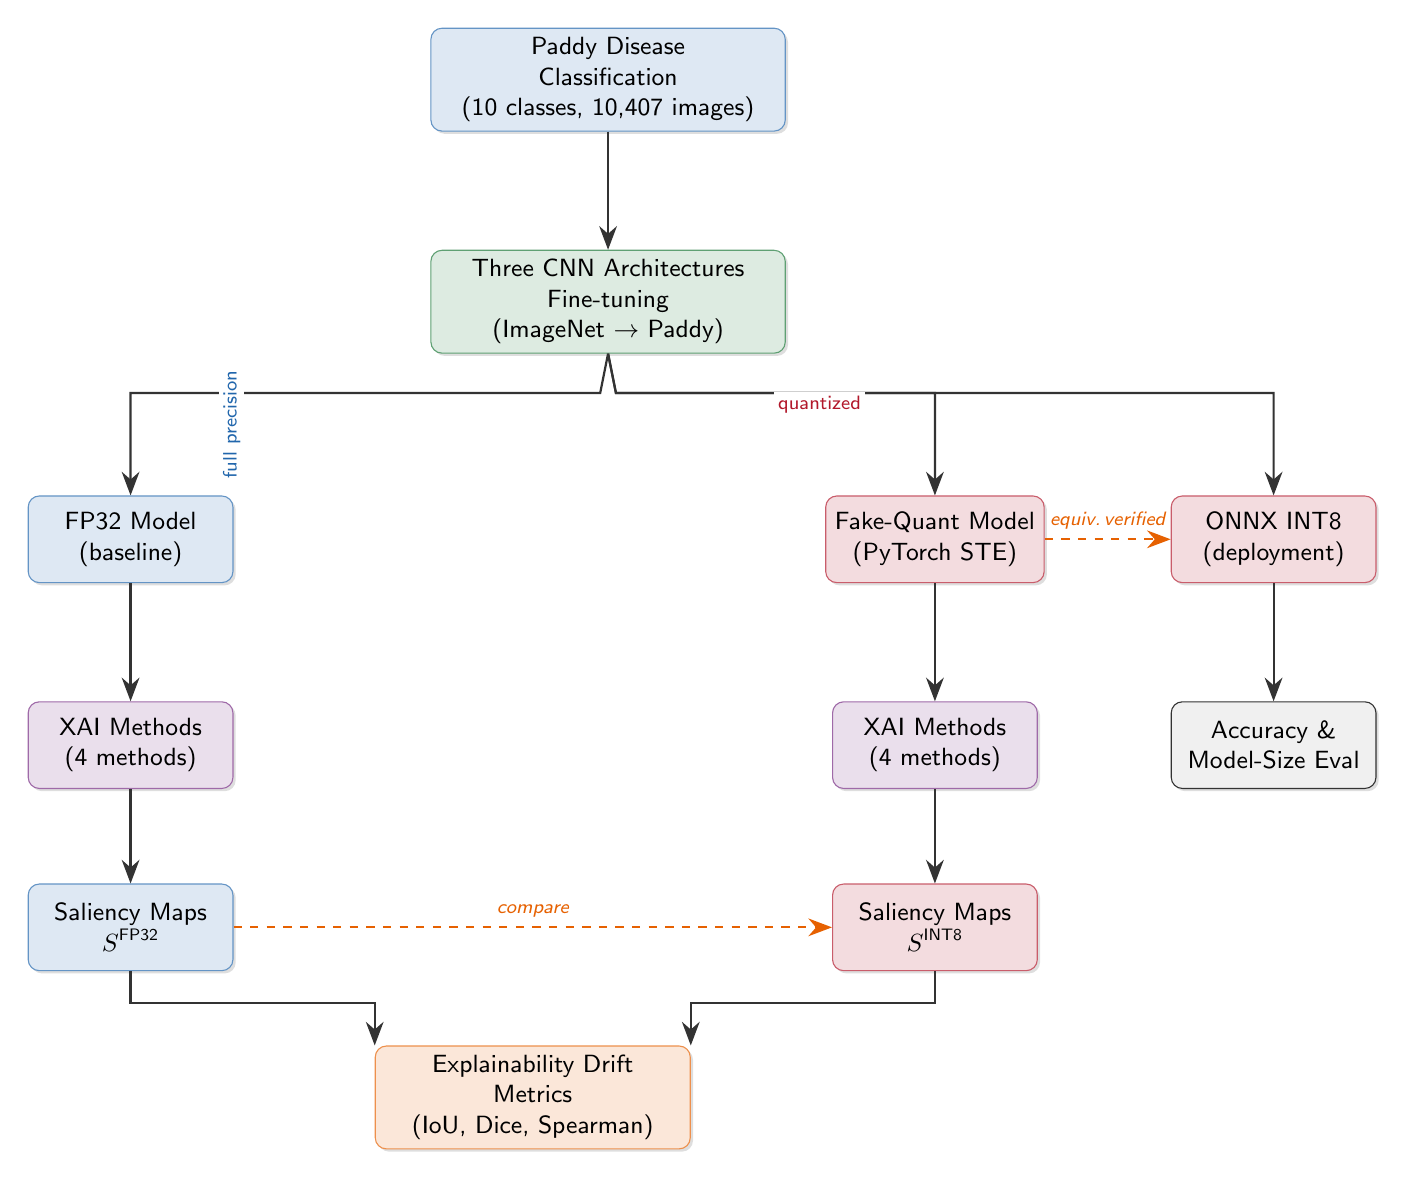
\begin{tikzpicture}[
    node distance=1.4cm and 1.6cm,
    every node/.style={font=\sffamily\small},
    block/.style={rectangle, draw=darktext, fill=lightgray, rounded corners=4pt,
                  minimum height=1.1cm, minimum width=2.6cm, align=center,
                  drop shadow={shadow xshift=1pt, shadow yshift=-1pt, fill=midgray}},
    fpblock/.style={block, fill=fpblue!15, draw=fpblue!70},
    intblock/.style={block, fill=intgreen!15, draw=intgreen!70},
    quantblock/.style={block, fill=quantred!15, draw=quantred!70},
    xaiblock/.style={block, fill=xaipurple!15, draw=xaipurple!70},
    driftblock/.style={block, fill=driftorange!15, draw=driftorange!70},
    myarrow/.style={-{Stealth[length=3mm]}, thick, darktext},
    mydasharrow/.style={-{Stealth[length=3mm]}, thick, dashed, driftorange},
]

% --- Row 1: Dataset ---
\node[fpblock, minimum width=4.5cm] (dataset) {Paddy Disease\\Classification\\(10 classes, 10{,}407 images)};

% --- Row 2: Model Training ---
\node[intblock, below=1.5cm of dataset, minimum width=4.5cm] (train) {Three CNN Architectures\\Fine-tuning\\(ImageNet $\rightarrow$ Paddy)};

% --- Row 3: FP32 and INT8 branches ---
\node[fpblock, below left=1.8cm and 2.5cm of train] (fp32) {FP32 Model\\(baseline)};
\node[quantblock, below right=1.8cm and 0.5cm of train] (fq) {Fake-Quant Model\\(PyTorch STE)};
\node[quantblock, right=1.6cm of fq] (onnx) {ONNX INT8\\(deployment)};

% --- Row 4: XAI ---
\node[xaiblock, below=1.5cm of fp32] (xaifp) {XAI Methods\\(4 methods)};
\node[xaiblock, below=1.5cm of fq] (xaiint) {XAI Methods\\(4 methods)};

% --- Row 4b: Deployment evaluation (ONNX branch) ---
\node[block, below=1.5cm of onnx, minimum width=2.6cm] (deploy) {Accuracy \&\\Model-Size Eval};

% --- Row 5: Saliency Maps ---
\node[fpblock, below=1.2cm of xaifp] (smfp) {Saliency Maps\\$S^{\text{FP32}}$};
\node[quantblock, below=1.2cm of xaiint] (smint) {Saliency Maps\\$S^{\text{INT8}}$};

% --- Row 6: Drift Metrics ---
\node[driftblock, below=1.5cm of $(smfp)!0.5!(smint)$, minimum width=4.0cm] (drift) {Explainability Drift\\Metrics\\(IoU, Dice, Spearman)};

% --- Arrows ---
\draw[myarrow] (dataset) -- (train);
\draw[myarrow] (train.south) -- ++(-0.1,-0.5) -| (fp32.north);
\draw[myarrow] (train.south) -- ++(0.1,-0.5) -| (fq.north);
\draw[myarrow] (train.south) -- ++(0.1,-0.5) -| (onnx.north);
\draw[myarrow] (fp32) -- (xaifp);
\draw[myarrow] (fq) -- (xaiint);
\draw[myarrow] (onnx) -- (deploy);
\draw[myarrow] (xaifp) -- (smfp);
\draw[myarrow] (xaiint) -- (smint);
\draw[myarrow] (smfp.south) -- ++(0,-0.4) -| (drift.north west);
\draw[myarrow] (smint.south) -- ++(0,-0.4) -| (drift.north east);

% --- Labels on branches ---
\node[font=\sffamily\scriptsize, fpblue, rotate=90, anchor=south, fill=white, inner sep=1.5pt] at ($(train.south west)!0.5!(fp32.north)+(-0.45,0)$) {full precision};
\node[font=\sffamily\scriptsize, quantred, anchor=west, fill=white, inner sep=1.5pt] at ($(train.south)+(2.1,-0.65)$) {quantized};

% --- Dashed equivalence arrow between fake-quant and ONNX ---
\draw[mydasharrow] (fq.east) -- node[above, font=\sffamily\scriptsize\itshape, driftorange]{equiv.\,verified} (onnx.west);

% --- Dashed comparison arrow ---
\draw[mydasharrow] (smfp.east) -- node[above, font=\sffamily\scriptsize\itshape, driftorange]{compare} (smint.west);

\end{tikzpicture}%
}
\caption{Quant-XAI experimental pipeline. Each trained model yields two quantized variants: an ONNX Runtime INT8 model for deployment evaluation (accuracy and model size), and a PyTorch fake-quantized model that simulates identical INT8 arithmetic while retaining gradient access for XAI computation (prediction equivalence verified between the two). Four post-hoc XAI methods generate saliency maps from both FP32 and fake-quantized models on identical evaluation images, and explanation drift is quantified using three complementary metrics.}
\label{fig:pipeline}
\end{figure}


Figure~\ref{fig:pipeline} illustrates the complete Quant-XAI experimental pipeline. Each component---dataset, model training, quantization, XAI computation, and drift measurement---is detailed in the subsections below.




\subsection*{Dataset and preprocessing}

The Paddy Disease Classification dataset\cite{PaddyDisease2022}, a publicly available benchmark for rice leaf disease detection, was selected for this study. The dataset comprises 10{,}407 high-resolution RGB photographs of rice (\emph{Oryza sativa}) paddy leaves, captured under field conditions and annotated by agricultural experts into 10 mutually exclusive classes reflecting distinct disease categories and healthy baseline (Table~\ref{tab:paddy_dist}).

\begin{table}[!ht]
\centering
\caption{Paddy Disease Classification dataset: class taxonomy and representative lesion patterns relevant to XAI saliency analysis.}
\label{tab:paddy_dist}
\begin{tabular}{clll}
\toprule
\textbf{Class ID} & \textbf{Disease} & \textbf{Lesion pattern} \\
\midrule
0 & Bacterial leaf blight & Linear water-soaked lesions \\
1 & Bacterial leaf streak & Narrow interveinal streaks \\
2 & Bacterial panicle blight & Panicle discolouration \\
3 & Blast & Diamond-shaped necrotic lesions \\
4 & Brown spot & Circular brown lesions with halos \\
5 & Dead heart & Central shoot dieback \\
6 & Downy mildew & Diffuse chlorotic patches \\
7 & Hispa & Tunnelled transparent patches \\
8 & Normal (healthy) & Uniform green, no lesions \\
9 & Tungro & Orange-yellow discolouration \\
\bottomrule
\end{tabular}
\end{table}

Lesion appearance varies across these classes, from localised high-contrast lesions (blast, brown spot) to diffuse low-contrast symptoms (downy mildew, tungro). We describe this variation because it is a property of the dataset, but we do not treat it as an explanatory variable: as reported below, class-level drift shows no significant association with class frequency, and per-class results are presented as exploratory only. The dataset provides no lesion-level annotations, so morphological hypotheses cannot be tested on it, and we address explanation quality separately using an externally annotated dataset.

Images were resized to $224 \times 224$ pixels and normalised using ImageNet channel statistics:
\[
\mu = [0.485,\, 0.456,\, 0.406], \quad \sigma = [0.229,\, 0.224,\, 0.225].
\]
The dataset was split into training~(80\%) and validation~(20\%) partitions via stratified sampling to preserve per-class proportions. Standard augmentations---random resized crop, horizontal flip, and normalisation---were applied during training.

\subsection*{Model architectures}

Three convolutional neural network architectures of varying complexity and design philosophy were selected to investigate how architectural choices interact with quantization-induced explanation drift:

\begin{enumerate}[leftmargin=1.5em, itemsep=2pt]
  \item \textbf{EfficientNetV2-S\cite{Tan2021efficientnetv2}:} compound-scaled architecture combining Fused-MBConv and standard MBConv blocks with squeeze-and-excitation (SE) attention, representing modern efficient design.
  \item \textbf{ResNet50\cite{He2016resnet}:} standard residual architecture with skip connections, representing the classical deep learning paradigm with well-understood gradient flow properties.
  \item \textbf{MobileNetV3-Large\cite{Howard2019mobilenetv3}:} depthwise-separable convolutions with hard-swish activations and SE blocks, representing ultra-efficient mobile-deployment architectures.
\end{enumerate}

All three models were initialised with ImageNet-1K pre-trained weights from the \texttt{timm} library\cite{Wightman2021timm}.

\subsection*{Training protocol and implementation details}

Each architecture was fine-tuned for 12 epochs with AdamW (learning rate $1 \times 10^{-3}$, weight decay $1 \times 10^{-4}$), a cosine annealing schedule with 3 warm-up epochs, batch size 48, cross-entropy loss, and bfloat16 automatic mixed precision. The checkpoint with the highest validation macro-F1 was retained; the selected epochs were 7 (EfficientNetV2-S), 11 (ResNet-50), and 9 (MobileNetV3-Large).

\textbf{Data partitioning.} The 10{,}407 images were split 80/20 into training and validation partitions by stratified sampling on the class label with a fixed seed, giving 8{,}325 training and 2{,}082 validation images. No image appears in more than one partition, and the same partition is reused for every architecture, quantization mode, explanation method, and QAT run reported in this paper.

\textbf{Explanation evaluation subset.} Computing four explanation methods on every validation image for every architecture and every quantization mode is not tractable: LIME alone requires 256 forward passes per image and Integrated Gradients requires 50. We therefore evaluate drift on a fixed, stratified random subset of 320 validation images (32 per class, $15.4\%$ of the validation split), drawn once with seed 42 and held constant across all architectures, methods, and modes so that every comparison is paired at the image level. LIME uses a 120-image stratified subset of the same 320 for the same reason. This yields $3 \times 320 \times 3 + 3 \times 120 = 3{,}240$ paired FP32--INT8 saliency comparisons per operating point, a 162$\times$ increase over the 20-image evaluation of the original submission. The power analysis reported below confirms this is sufficient for the effect sizes observed.

\textbf{Determinism and seeds.} Python, NumPy, and PyTorch random number generators are seeded from a single configuration value. The primary seed is 42; seed replication for the drift and QAT results uses 42, 1337, and 2024. Because cuDNN autotuning and atomic reductions are not bit-deterministic on GPU, we report seed-to-seed variability explicitly rather than claiming exact reproducibility.

\textbf{Preprocessing common grid.} All saliency maps, regardless of method or native resolution, are bilinearly resampled to a common $224 \times 224$ grid before any metric is computed, and are min--max normalised to $[0,1]$. Grad-CAM and Grad-CAM++ maps are produced at the $7 \times 7$ resolution of the target activation and upsampled; Integrated Gradients and LIME are natively at input resolution. Fixing the comparison grid ensures that IoU, Dice, and Spearman $\rho$ are computed over an identical number of elements ($N = 50{,}176$) for every method, so that top-$k$ thresholds and rank statistics are directly comparable.

\textbf{Software and hardware.} All experiments ran in a single Kaggle session on one NVIDIA Tesla T4 GPU (16\,GB, compute capability 7.5) with CUDA 12.8, using PyTorch 2.10.0, timm 1.0.26, ONNX 1.22.0, ONNX Runtime 1.28.0, NumPy 2.0.2, pandas 2.3.3, SciPy 1.16.3, scikit-learn 1.6.1, scikit-image 0.25.2, and Matplotlib 3.10.0 under Python 3.12. Exact pinned versions are recorded in the archived environment manifest. Total wall-clock time for the complete pipeline was approximately 4.5 hours.

\subsection*{INT8 post-training quantization}

Each trained FP32 model was exported to ONNX (opset~17) and quantized with the ONNX Runtime static quantization path (Figure~\ref{fig:quantization}), inserting Quantize-Dequantize (QDQ) nodes with symmetric per-channel weight quantization and asymmetric per-tensor activation quantization. All three architectures quantized through the static path without dynamic fallback (Table~\ref{tab:quant_config}).

\textbf{Calibration subset specification.} The calibration set is drawn exclusively from the \emph{training} partition, never from validation, and comprises 512 images sampled stratified by class (51--52 images per class) with seed 42. Calibration images pass through the identical deterministic preprocessing applied at inference (resize to $224 \times 224$, ImageNet channel normalisation) with all stochastic augmentation disabled. The same fixed calibration subset is reused for every architecture. Within the ONNX Runtime calibration-method ablation the per-arm calibration sizes are not equal, as reported in Table~\ref{tab:calib_ablation}; we therefore repeat all three calibrators at a single matched budget in Table~\ref{tab:calib_matched} so that differences between calibrators are attributable to the algorithm rather than to the amount of calibration data. We note as a correction that the version of this study originally submitted drew the calibration subset from the validation split; that configuration leaks evaluation data into quantization parameters, and we quantify its effect explicitly in Table~\ref{tab:calib_ablation}.

\textbf{Calibration method ablation.} Because activation ranges determine the entire INT8 operating point, we ablate three ONNX Runtime calibrators, MinMax, entropy, and percentile, alongside the 512-image PyTorch fake-quantization configuration (Table~\ref{tab:calib_ablation}). Within that table the ONNX Runtime MinMax arm is calibrated on the full 512-image subset while the entropy and percentile arms are calibrated on a 64-image cap, so calibrator identity and calibration-set size are not separated inside it. Because the comparison of interest is between calibrators, we additionally rebuild all three at one identical matched calibration budget (Table~\ref{tab:calib_matched}), which removes that confound and leaves the ordering we rely on unchanged. MinMax is the ONNX Runtime default and the setting described in the original submission, but it is not robust: a single outlying activation widens the quantization range and coarsens every other value. We report percentile calibration as the deployed configuration and retain the MinMax result as the negative control.

For explanation evaluation, which requires gradient access that the ONNX Runtime inference engine does not expose, a matched fake-quantized model is constructed in PyTorch as described below.


% ============================================================================
% FIGURE 3 — Quantization Process Diagram (TikZ)
% ============================================================================
\begin{figure}[!ht]
\centering
\resizebox{0.92\textwidth}{!}{%
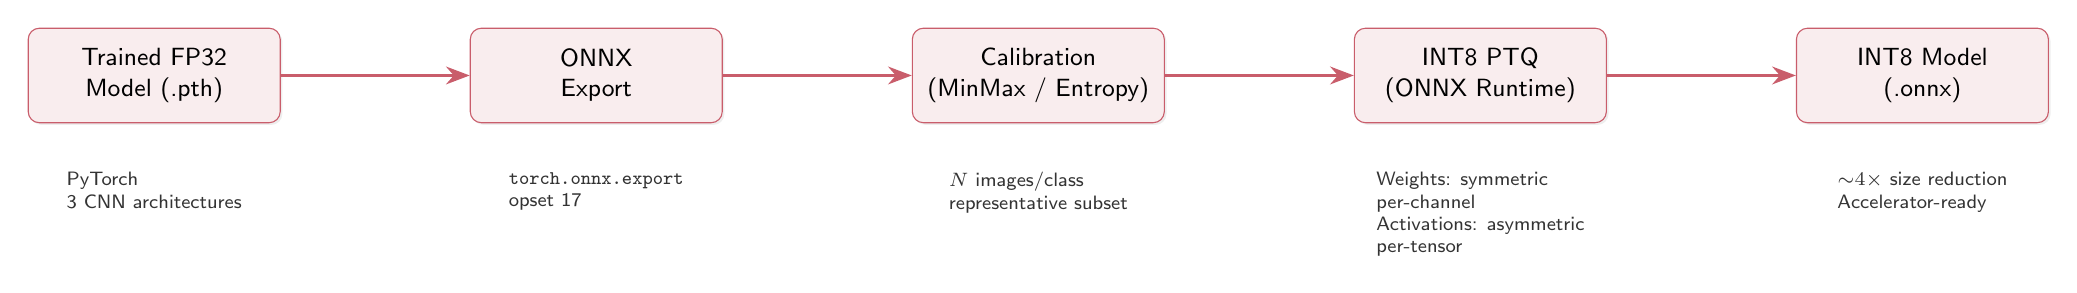
\begin{tikzpicture}[
    node distance=1.0cm and 2.4cm,
    every node/.style={font=\sffamily\small},
    stepbox/.style={rectangle, draw=quantred!70, fill=quantred!8,
                 rounded corners=4pt, minimum height=1.2cm,
                 minimum width=3.2cm, align=center,
                 drop shadow={shadow xshift=0.8pt, shadow yshift=-0.8pt, fill=midgray!50}},
    detailtext/.style={font=\sffamily\scriptsize, align=left, text=darktext},
    myarrow/.style={-{Stealth[length=3mm]}, very thick, quantred!70},
]

\node[stepbox] (s1) {Trained FP32\\Model (.pth)};
\node[stepbox, right=of s1] (s2) {ONNX\\Export};
\node[stepbox, right=of s2] (s3) {Calibration\\(MinMax / Entropy)};
\node[stepbox, right=of s3] (s4) {INT8 PTQ\\(ONNX Runtime)};
\node[stepbox, right=of s4] (s5) {INT8 Model\\(.onnx)};

\draw[myarrow] (s1) -- (s2);
\draw[myarrow] (s2) -- (s3);
\draw[myarrow] (s3) -- (s4);
\draw[myarrow] (s4) -- (s5);

% Detail annotations
\node[detailtext, below=0.5cm of s1] {PyTorch\\3 CNN architectures};
\node[detailtext, below=0.5cm of s2] {\texttt{torch.onnx.export}\\opset 17};
\node[detailtext, below=0.5cm of s3] {$N$ images/class\\representative subset};
\node[detailtext, below=0.5cm of s4] {Weights: symmetric\\per-channel\\Activations: asymmetric\\per-tensor};
\node[detailtext, below=0.5cm of s5] {${\sim}4\times$ size reduction\\Accelerator-ready};

\end{tikzpicture}%
}
\caption{INT8 post-training quantization pipeline. The trained FP32 model is exported to ONNX format, calibrated with a representative image subset, and quantized to INT8 via the ONNX Runtime quantization toolkit.}
\label{fig:quantization}
\end{figure}


\subsection*{Grad-CAM target layer resolution}

Grad-CAM and Grad-CAM++ require a target activation tensor with non-trivial spatial extent. In applied work the target is often described only as ``the last convolutional layer'', and is selected in practice by taking the last four-dimensional module of the network. We find that this heuristic fails for all three architectures studied here, and that the failure is the dominant confound in measuring explanation drift.

In \texttt{timm} implementations, the module that a naive traversal returns is the global pooling output for EfficientNetV2-S and ResNet-50 (\texttt{global\_pool.pool}, shapes $1 \times 1280 \times 1 \times 1$ and $1 \times 2048 \times 1 \times 1$) and the post-pooling projection \texttt{act2} for MobileNetV3-Large ($1 \times 1280 \times 1 \times 1$). All three emit a $1 \times 1$ spatial map. A class activation map computed from a $1 \times 1$ tensor is by construction a single scalar broadcast over the image: it is spatially constant, carries no localisation information, and yields tied ranks at every pixel. MobileNetV3-Large is affected most severely because \texttt{timm} applies global pooling \emph{before} the final $1 \times 1$ projection, so even the last convolution-like module is post-pooling.

We therefore resolve the target layer by an explicit, architecture-agnostic criterion: traverse named modules in forward order, record the output shape of each under a single dummy forward pass, and select the last module whose output is four-dimensional with both spatial dimensions at least 4. This resolves to \texttt{bn2} ($1 \times 1280 \times 7 \times 7$) for EfficientNetV2-S, \texttt{layer4} ($1 \times 2048 \times 7 \times 7$) for ResNet-50, and \texttt{blocks} ($1 \times 960 \times 7 \times 7$) for MobileNetV3-Large (Table~\ref{tab:cam_layers}). Hooks are registered on the resolved module in both the FP32 teacher and the fake-quantized student, so the two saliency maps being compared are always taken from the same named module at the same depth.

To separate this artefact from genuine quantization sensitivity we additionally sweep drift over every candidate layer in the terminal stage of each network (Table~\ref{tab:cam_layer_sweep}). Throughout the paper, results computed with the naive degenerate target are reported under the label \emph{legacy} and results computed with the resolved target under \emph{QDQ}; the legacy condition is retained deliberately, because it reproduces and explains the attribution collapse reported in the original version of this study.

\subsection*{XAI method implementations}

Four post-hoc explanation methods were applied to identical evaluation images for both FP32 and fake-quantized models (Figure~\ref{fig:xai_methods}):

\begin{enumerate}[leftmargin=1.5em, itemsep=2pt]
  \item \textbf{Grad-CAM\cite{Selvaraju2017gradcam}:} gradient-weighted class activation maps computed from the resolved target activation (Table~\ref{tab:cam_layers}) via forward and backward PyTorch hooks, with channel weights obtained by global average pooling of the gradient of the target-class logit, followed by ReLU and bilinear upsampling to $224 \times 224$. The explained class is always the FP32 model's predicted class, held fixed for the INT8 model so that both maps explain the same decision.
  \item \textbf{Grad-CAM++\cite{Chattopadhay2018gradcampp}:} pixel-wise weighting using second- and third-order derivatives; same target layer as Grad-CAM.
  \item \textbf{Integrated Gradients\cite{Sundararajan2017ig}:} attribution via path integral from a black baseline ($\mathbf{0}$) to the input image; 50 interpolation steps.
  \item \textbf{LIME\cite{Ribeiro2016lime}:} Local Interpretable Model-agnostic Explanations with 256 perturbed samples per image and quickshift superpixel segmentation.
\end{enumerate}

To ensure a methodologically valid comparison, all four XAI methods must be applied identically to both FP32 and quantized models. Since the ONNX Runtime inference engine used for INT8 deployment does not expose gradient computation, we employ PyTorch's fake-quantization framework to simulate INT8 post-training quantization while retaining full gradient flow. Specifically, the trained FP32 model is instrumented with \texttt{FakeQuantize} modules on all weight and activation tensors, configured to match the ONNX Runtime PTQ settings (symmetric per-channel weight quantization, asymmetric per-tensor activation quantization, MinMax calibration). During the forward pass, these modules simulate INT8 rounding and clamping; during backpropagation, gradients propagate through the straight-through estimator (STE)\cite{Jacob2018quantization}, enabling Grad-CAM, Grad-CAM++, and Integrated Gradients to be computed using identical implementations on both FP32 and fake-quantized models. Drift in gradient-based attributions therefore arises from quantization-induced changes to intermediate activations and weight values, not from methodological differences in attribution computation. LIME, being inherently model-agnostic, is applied identically to both model variants without modification.

\textbf{Prediction equivalence verification.} To confirm that the fake-quantized PyTorch model faithfully represents the deployed ONNX Runtime INT8 model, we evaluated the FP32 model, the fake-quantized model, and the exported ONNX Runtime INT8 graph under all three calibrators on the full validation set (2{,}082 images). Per-architecture top-1 agreement on the full split, mean and maximum absolute logit differences, logit cosine similarity, and layer-wise centred kernel alignment between FP32 and INT8 intermediate features are reported in Table~\ref{tab:equivalence}, together with the corresponding subset values, so that the simulated and deployed realisations can be compared directly rather than assumed equivalent.


% ============================================================================
% FIGURE 2 — XAI Methods Overview Diagram (TikZ)
% ============================================================================
\begin{figure}[!ht]
\centering
\resizebox{\textwidth}{!}{%
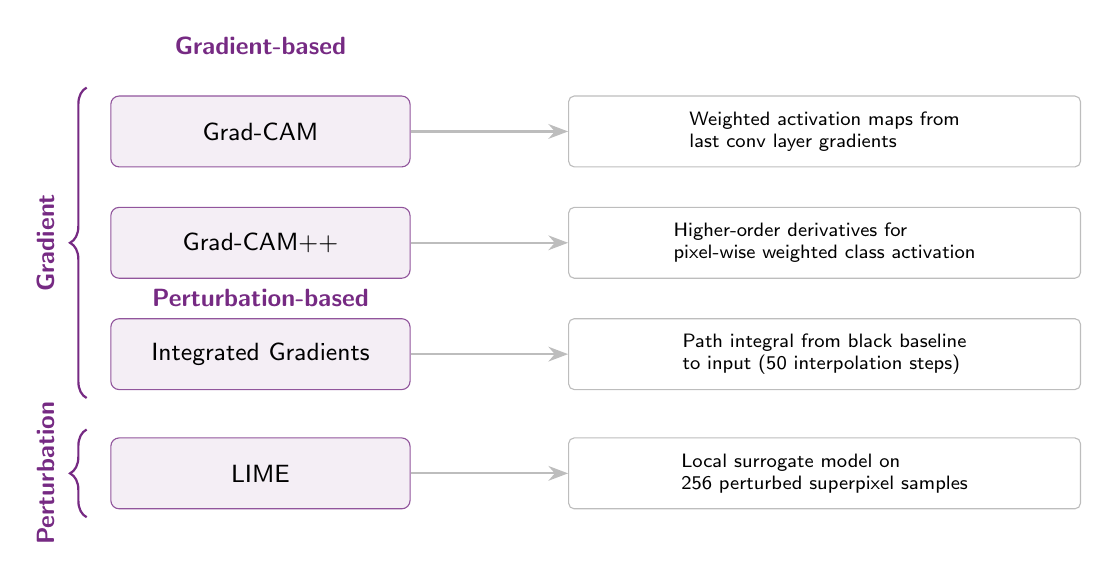
\begin{tikzpicture}[
    node distance=0.8cm and 2.0cm,
    every node/.style={font=\sffamily\small},
    method/.style={rectangle, draw=xaipurple!80, fill=xaipurple!8,
                   rounded corners=3pt, minimum height=0.9cm,
                   minimum width=3.8cm, align=center},
    desc/.style={rectangle, draw=midgray, fill=white,
                 rounded corners=2pt, minimum height=0.9cm,
                 minimum width=6.5cm, align=left,
                 font=\sffamily\scriptsize},
    cat/.style={font=\sffamily\bfseries\small, xaipurple},
    myarrow/.style={-{Stealth[length=2.5mm]}, thick, midgray},
]

% Category labels
\node[cat] (grad) at (0,0) {Gradient-based};
\node[cat] (pert) at (0,-3.2) {Perturbation-based};

% Gradient-based methods
\node[method, below=0.4cm of grad] (gc) {Grad-CAM};
\node[desc, right=of gc] (gcd) {Weighted activation maps from\\last conv layer gradients};

\node[method, below=0.5cm of gc] (gcpp) {Grad-CAM++};
\node[desc, right=of gcpp] (gcppd) {Higher-order derivatives for\\pixel-wise weighted class activation};

\node[method, below=0.5cm of gcpp] (ig) {Integrated Gradients};
\node[desc, right=of ig] (igd) {Path integral from black baseline\\to input (50 interpolation steps)};

% Perturbation-based methods
\node[method, below=0.6cm of ig] (lime) {LIME};
\node[desc, right=of lime] (limed) {Local surrogate model on\\256 perturbed superpixel samples};

% Arrows
\draw[myarrow] (gc) -- (gcd);
\draw[myarrow] (gcpp) -- (gcppd);
\draw[myarrow] (ig) -- (igd);
\draw[myarrow] (lime) -- (limed);

% Braces
\draw[decorate, decoration={brace, amplitude=6pt, mirror}, xaipurple, thick]
  ($(gc.north west)+(-0.3,0.1)$) -- ($(ig.south west)+(-0.3,-0.1)$)
  node[midway, left=8pt, cat, rotate=90, anchor=south] {Gradient};

\draw[decorate, decoration={brace, amplitude=6pt, mirror}, xaipurple, thick]
  ($(lime.north west)+(-0.3,0.1)$) -- ($(lime.south west)+(-0.3,-0.1)$)
  node[midway, left=8pt, cat, rotate=90, anchor=south] {Perturbation};

\end{tikzpicture}%
}
\caption{Four post-hoc XAI methods evaluated in this study. Three gradient-based methods (Grad-CAM, Grad-CAM++, Integrated Gradients) and one perturbation-based method (LIME) are applied identically to both FP32 and INT8 model variants.}
\label{fig:xai_methods}
\end{figure}


\subsection*{Explainability drift metrics}

For each evaluation image $i$, the FP32 saliency map $S_i^{\text{FP32}}$ and fake-quantized saliency map $S_i^{\text{INT8}}$ (both min-max normalised to $[0,1]$) were compared using three complementary metrics (Figure~\ref{fig:drift_metrics}):

\textbf{Choice of $k$ and sensitivity.} Top-$k$ metrics require a threshold, and any single choice is arbitrary. We report $k = 0.15$ as the primary operating point because it is the midpoint of the $0.10$--$0.20$ fractional lesion area typical of this dataset, but we do not rely on it: every drift metric is recomputed over $k \in \{0.05, 0.10, 0.15, 0.20, 0.25, 0.30\}$ (Table~\ref{tab:k_sweep}, Figure~\ref{fig:k_sweep}), and we quantify whether conclusions depend on $k$ using Kendall's $\tau$ between the method ranking at each $k$ and the ranking at the primary $k$ (Table~\ref{tab:rank_stability}). Absolute overlap necessarily increases with $k$ because the random-overlap baseline itself increases, so all top-$k$ values are interpreted as ratios to that baseline rather than in absolute terms.

\textbf{Random-overlap baselines.} For two independent random binary masks each selecting a fraction $k$ of $N$ elements, the expected overlap statistics are
\begin{equation}
\mathbb{E}[\text{IoU}] = \frac{k}{2-k}, \qquad \mathbb{E}[\text{Dice}] = k,
\label{eq:chance}
\end{equation}
giving $\mathbb{E}[\text{IoU}] = 0.081$ and $\mathbb{E}[\text{Dice}] = 0.150$ at $k = 0.15$. We confirm these analytic values empirically by Monte Carlo simulation over matched mask sizes (Table~\ref{tab:chance}) and report every measured overlap alongside its ratio to chance. Without this baseline a top-$k$ IoU of $0.15$ would appear to indicate meaningful agreement when it is in fact indistinguishable from random.

\textbf{Top-$k$ Intersection-over-Union (IoU).} Both maps were binarised at the top-$k$\% threshold, retaining only the most salient $k$\% of pixels. IoU was computed between the resulting binary masks:
\begin{equation}
\text{IoU}_k = \frac{|B_k^{\text{FP32}} \cap B_k^{\text{INT8}}|}{|B_k^{\text{FP32}} \cup B_k^{\text{INT8}}|}
\label{eq:iou}
\end{equation}
This metric captures spatial overlap of the highest-activation regions and is sensitive to localised shifts in saliency focus.

\textbf{Top-$k$ Dice Coefficient.} The Dice coefficient (F1 score of spatial overlap) is computed on the same binarised masks:
\begin{equation}
\text{Dice}_k = \frac{2|B_k^{\text{FP32}} \cap B_k^{\text{INT8}}|}{|B_k^{\text{FP32}}| + |B_k^{\text{INT8}}|}
\label{eq:dice}
\end{equation}
We note explicitly that top-$k$ IoU and top-$k$ Dice are not independent evidence. Because top-$k$ binarisation fixes $|B_k^{\text{FP32}}| = |B_k^{\text{INT8}}| = kN$, the two statistics are related deterministically by $\text{Dice}_k = 2\,\text{IoU}_k / (1 + \text{IoU}_k)$, a strictly monotone transform. Reporting both is retained only for comparability with prior segmentation-style literature; they constitute a single spatial-overlap axis, and Spearman $\rho$ is the only metric here that carries genuinely independent information about attribution structure.

\textbf{Spearman Rank Correlation ($\rho$).} The Spearman rank correlation between the flattened, continuous-valued saliency maps quantifies whether the \emph{relative ordering} of pixel attributions is preserved under quantization:
\begin{equation}
\rho = 1 - \frac{6\sum_{j=1}^{N} d_j^2}{N(N^2 - 1)}
\label{eq:spearman}
\end{equation}
where $d_j$ is the difference in ranks of pixel $j$ between the two maps, computed with midrank correction for tied values. A correlation of $\rho = 1$ indicates perfect rank preservation and $\rho = 0$ indicates no monotonic relationship.

\textbf{Tie handling and collapse are reported separately from $\rho$.} If either map is constant, its ranks are all tied, its variance is zero, and Spearman $\rho$ is mathematically \emph{undefined} rather than zero. Assigning $\rho = 0$ in that situation, as the original version of this study did, conflates two categorically different outcomes: an explanation that has been re-ordered arbitrarily, and an explanation that has ceased to exist. We therefore adopt the following rule throughout. A saliency map is labelled \emph{collapsed} when the number of distinct values it contains falls below a fixed threshold, evaluated as a count of unique quantised levels; collapsed maps are excluded from the $\rho$ distribution and reported instead as a \emph{collapse rate}, the fraction of images on which the condition occurs. This yields two reported quantities, a collapse rate and a Spearman distribution over non-degenerate maps, and the number of maps entering each is stated for every condition. Under the resolved target layers, the collapse rate is $0.000$ for all 24 architecture--method--metric conditions and all $3{,}240$ comparisons enter the $\rho$ distribution; under the degenerate target layers examined in Table~\ref{tab:cam_layer_sweep} the collapse rate is non-zero and is reported as such. Concretely, a saliency map is classified as collapsed when it contains fewer than two distinct values or its spatial standard deviation falls below $10^{-6}$; these are the thresholds behind every collapse count reported in this paper.


% ============================================================================
% FIGURE 4 — Drift Metrics Conceptual Diagram (TikZ)
% ============================================================================
\begin{figure}[!ht]
\centering
\resizebox{0.95\textwidth}{!}{%
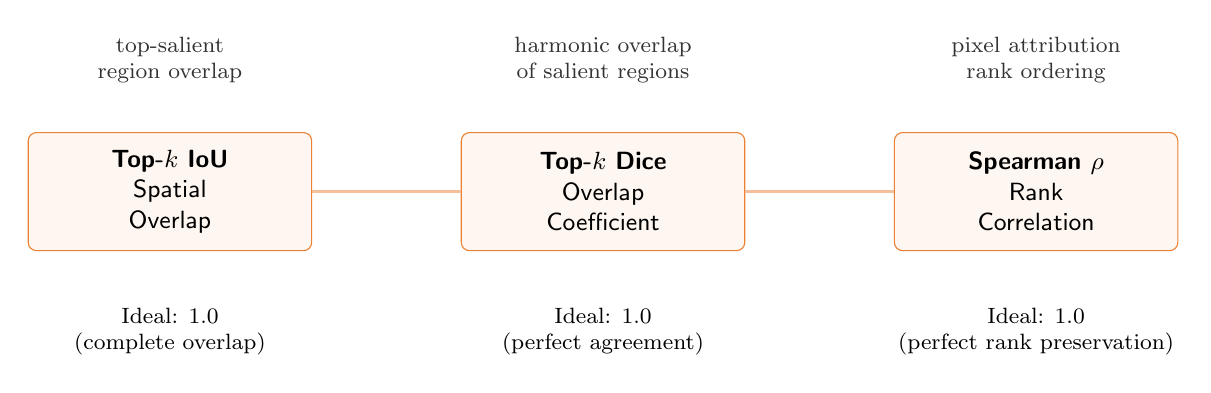
\begin{tikzpicture}[
    every node/.style={font=\sffamily\small},
    metricbox/.style={rectangle, draw=driftorange!80, fill=driftorange!6,
                      rounded corners=3pt, minimum height=1.5cm,
                      minimum width=3.6cm, align=center},
    formula/.style={font=\footnotesize, align=center},
    heading/.style={font=\sffamily\bfseries, driftorange},
]

\node[metricbox] (iou)  at (0,0) {\textbf{Top-$k$ IoU}\\Spatial\\Overlap};
\node[metricbox] (dice) at (5.5,0) {\textbf{Top-$k$ Dice}\\Overlap\\Coefficient};
\node[metricbox] (spearman) at (11.0,0) {\textbf{Spearman $\rho$}\\Rank\\Correlation};

% Ideal targets
\node[formula, below=0.6cm of iou]  {Ideal: 1.0\\(complete overlap)};
\node[formula, below=0.6cm of dice] {Ideal: 1.0\\(perfect agreement)};
\node[formula, below=0.6cm of spearman] {Ideal: 1.0\\(perfect rank preservation)};

% What each captures
\node[formula, above=0.5cm of iou, text=darktext]  {top-salient\\region overlap};
\node[formula, above=0.5cm of dice, text=darktext]  {harmonic overlap\\of salient regions};
\node[formula, above=0.5cm of spearman, text=darktext]  {pixel attribution\\rank ordering};

% Connecting line
\draw[driftorange!40, very thick] (iou.east) -- (dice.west);
\draw[driftorange!40, very thick] (dice.east) -- (spearman.west);

\end{tikzpicture}%
}
\caption{Explainability drift metrics used to quantify saliency-map divergence. Top-$k$ IoU and top-$k$ Dice measure spatial overlap of the most salient regions; Spearman~$\rho$ quantifies rank-order preservation of pixel attributions.}
\label{fig:drift_metrics}
\end{figure}


\subsection*{XAI-preserving quantization-aware training}

To mitigate explanation drift we use quantization-aware training (QAT) with a teacher--student CAM consistency loss. The FP32-trained model is frozen and serves as the teacher; a copy with fake-quantize nodes inserted on weights and activations serves as the student. The combined loss is:
\begin{equation}
\mathcal{L}_{\text{QAT}} = \mathcal{L}_{\text{CE}} + \lambda \cdot \text{MSE}\bigl(\text{CAM}_{\text{teacher}},\, \text{CAM}_{\text{student}}\bigr)
\label{eq:qat}
\end{equation}
where $\mathcal{L}_{\text{CE}}$ is cross-entropy, MSE is mean squared error over the spatial map, and $\lambda$ weights explanation preservation against classification accuracy. The following details were requested and are specified here in full.

\textbf{CAM computation inside the loss.} Both teacher and student CAMs are Grad-CAM maps taken from the same resolved target module (Table~\ref{tab:cam_layers}) at $7 \times 7$ resolution, min--max normalised per image to $[0,1]$ before the MSE is taken, so the loss constrains spatial shape and not activation magnitude.

\textbf{Target class selection.} The consistency term is computed at the \emph{ground-truth} class of each training image, not the student's argmax. Using the student's prediction would make the regularisation target move with the student and would reward degenerate agreement early in training when the student is still inaccurate.

\textbf{Gradient handling.} The teacher is held in evaluation mode with parameters frozen and its CAM is detached from the graph, so it acts as a fixed target. The student CAM requires a gradient-of-a-gradient path: the CAM depends on $\partial y_c / \partial A$, so backpropagating the MSE term requires second-order differentiation, and the inner backward pass is therefore taken with the graph retained. Gradients reach the quantized weights through the straight-through estimator, in which the fake-quantize operation is treated as identity on the backward pass within the clipping range and as zero outside it.

\textbf{Weight $\lambda$ and its control.} Rather than assert a single value, we sweep $\lambda \in \{0.0, 0.1, 0.5, 1.0, 2.0\}$ and report the full dose--response (Table~\ref{tab:lambda_sweep}, Figure~\ref{fig:lambda_sweep}). The $\lambda = 0$ arm is the essential control: it is identical to standard QAT in every respect except that the consistency term is switched off, so any effect attributed to explanation-aware QAT must exceed it. $\lambda = 0.5$ is reported as the primary setting and is replicated at seeds 42, 1337, and 2024.

\textbf{Schedule and re-evaluation.} The student is fine-tuned for 3 epochs on a $50\%$ stratified subsample of the training partition with AdamW at learning rate $1 \times 10^{-4}$. After training, the student is re-quantized and drift is recomputed on the identical 320-image evaluation subset and identical target layers used for the baseline, and classification performance is re-benchmarked on the validation split (Table~\ref{tab:post_qat}).

\subsection*{Statistical analysis}

All drift metrics are reported as mean $\pm$ standard deviation over the evaluation subset, together with the number of paired comparisons contributing to each estimate. At the primary operating point ($k = 0.15$, resolved target layers) the analysis comprises 3{,}240 paired FP32--INT8 comparisons.

\textbf{Interval estimates.} Two-sided $95\%$ confidence intervals for every architecture--method--metric cell are obtained by nonparametric bootstrap resampling of images with replacement, preserving the FP32--INT8 pairing within each resample. Intervals are reported as percentiles of the resampled mean distribution and are used to judge whether a cell exceeds its random-overlap baseline.

\textbf{Hypothesis tests.} Comparisons between explanation methods are paired at the image level, since every method is evaluated on the same images. We report the mean paired difference, Cohen's $d_z$ for paired designs, Cliff's $\delta$ as a distribution-free effect size, and two-sided $p$-values. Because six pairwise method comparisons and nine QAT comparisons are performed, all $p$-values are adjusted by the Holm--Bonferroni step-down procedure, and we report both raw and adjusted values.

\textbf{Power.} We compute the sample size required for $80\%$ power at representative effect sizes and the achieved power at the realised sample size, and we flag any comparison whose achieved power falls below $0.80$ rather than presenting it as a settled result.

\textbf{Replication and sanity checks.} The primary drift configuration is replicated at three independent training seeds (42, 1337, 2024) and seed-to-seed dispersion is reported. As a sanity check on the attribution pipeline, we also perform a cascading parameter-randomisation test, progressively replacing trained weights with random values and measuring the rank correlation between the resulting saliency map and that of the trained model; a faithful attribution method should lose correspondence as randomisation increases.

\textbf{Matched-prediction control.} To separate drift in the explanation mechanism from drift in the explained decision, all metrics are additionally computed on the matched-prediction subset, in which FP32 and INT8 models agree on the predicted class. Throughout, the explained class is fixed to the FP32 prediction for both models, so a change in the INT8 argmax does not silently change the quantity being explained.

\textbf{Reported improvement.} Relative change is computed as $\Delta = (m_{\text{mitigated}} - m_{\text{baseline}}) / |m_{\text{baseline}}| \times 100\%$. We report relative change only alongside the absolute values it derives from, because a large relative change on a near-zero baseline is not evidence of a practically meaningful effect.


% ============================================================================
% RESULTS
% ============================================================================
\section*{Results}

\subsection*{FP32 baselines and deployment cost}

All three architectures reach comparable accuracy on the validation split (Table~\ref{tab:fp32_baseline}), with macro-F1 between $0.971$ and $0.980$. Because the three models are within one percentage point of each other, subsequent differences in explanation drift cannot be attributed to differences in classification quality.

\begin{table}[!ht]
\centering
\caption{FP32 baseline classification performance on the validation split (2{,}082 images, 10 classes).}
\label{tab:fp32_baseline}
\begin{tabular}{lcccc}
\toprule
\textbf{Architecture} & \textbf{Macro-F1} & \textbf{Balanced Acc.} & \textbf{Accuracy} & \textbf{Best Epoch} \\
\midrule
EfficientNetV2-S  & \textbf{0.9796} & \textbf{0.9767} & \textbf{0.9793} & 7 \\
ResNet-50         & 0.9709 & 0.9688 & 0.9745 & 11 \\
MobileNetV3-Large & 0.9732 & 0.9696 & 0.9750 & 9 \\
\bottomrule
\end{tabular}
\end{table}

Table~\ref{tab:efficiency} reports parameter counts, multiply--accumulate cost, and measured latency, which were requested to substantiate claims about deployment efficiency. Two observations matter for interpreting the drift results. First, INT8 compression is close to the theoretical $4\times$ for all three models ($3.54$--$3.91\times$). Second, compression does not imply acceleration: MobileNetV3-Large is the smallest and cheapest model in FLOPs, yet its INT8 graph is \emph{slower} than its FP32 graph on CPU ($0.67\times$ speedup, i.e.\ $5.58 \rightarrow 8.30$\,ms), because the quantize and dequantize nodes surrounding its many lightweight depthwise operators cost more than the integer arithmetic saves. Efficiency claims for depthwise-separable architectures under INT8 therefore require measurement rather than assumption.

\begin{table}[!ht]
\centering
\scriptsize
\caption{Model complexity and measured deployment cost. GFLOPs are per image at $224 \times 224$. Latency is ONNX Runtime CPU, batch size 1. Speedup ${<}1$ indicates INT8 is slower than FP32.}
\label{tab:efficiency}
\setlength{\tabcolsep}{4pt}
\begin{tabular}{lcc cc c cc c}
\toprule
 & & & \multicolumn{3}{c}{\textbf{ONNX model size (MB)}} & \multicolumn{3}{c}{\textbf{ORT CPU latency (ms)}} \\
\cmidrule(lr){4-6} \cmidrule(lr){7-9}
\textbf{Architecture} & \textbf{Params (M)} & \textbf{GFLOPs} & \textbf{FP32} & \textbf{INT8} & \textbf{Comp.} & \textbf{FP32} & \textbf{INT8} & \textbf{Speedup} \\
\midrule
EfficientNetV2-S & 20.19 & 5.697 & 80.7 & 22.8 & 3.54$\times$ & 43.5 & 39.8 & 1.09$\times$ \\
ResNet-50 & 23.53 & 8.174 & 94.0 & 24.0 & 3.91$\times$ & 40.7 & 31.8 & 1.28$\times$ \\
MobileNetV3-L & 4.21 & 0.431 & 16.9 & 4.7 & 3.59$\times$ & 5.6 & 8.3 & 0.67$\times$ \\
\bottomrule
\end{tabular}
\end{table}

\subsection*{Grad-CAM target-layer selection, not quantization, produces attribution collapse}

This is the finding that reframes the study. Table~\ref{tab:cam_layers} contrasts the target layer resolved by the spatial-dimension criterion with the module returned by the naive ``last four-dimensional layer'' heuristic. For all three architectures the naive choice is degenerate: it emits a $1 \times 1$ spatial tensor and therefore cannot encode localisation at all.

\begin{table}[!ht]
\centering
\scriptsize
\caption{Resolved versus naive Grad-CAM target layers. The naive heuristic returns a globally pooled $1 \times 1$ tensor for every architecture, which forces a spatially constant class activation map.}
\label{tab:cam_layers}
\setlength{\tabcolsep}{4pt}
\begin{tabular}{lll ll}
\toprule
 & \multicolumn{2}{c}{\textbf{Resolved target}} & \multicolumn{2}{c}{\textbf{Naive target}} \\
\cmidrule(lr){2-3} \cmidrule(lr){4-5}
\textbf{Architecture} & \textbf{Module} & \textbf{Output shape} & \textbf{Module} & \textbf{Output shape} \\
\midrule
EfficientNetV2-S & \texttt{bn2} & (1, 1280, 7, 7) & \texttt{global\_pool.pool} & (1, 1280, 1, 1) \\
ResNet-50 & \texttt{layer4} & (1, 2048, 7, 7) & \texttt{global\_pool.pool} & (1, 2048, 1, 1) \\
MobileNetV3-L & \texttt{blocks} & (1, 960, 7, 7) & \texttt{act2} & (1, 1280, 1, 1) \\
\bottomrule
\end{tabular}
\end{table}

The consequence is quantified in Table~\ref{tab:cam_layer_sweep}, which sweeps every candidate layer in the terminal stage of each network. Within each architecture, all layers that satisfy the spatial criterion produce zero collapse and high rank preservation. The degenerate layers, shaded in the table, produce collapse rates of $0.408$ (EfficientNetV2-S, \texttt{global\_pool.pool}), $0.225$ (ResNet-50, \texttt{global\_pool.pool}), and $0.617$ (MobileNetV3-Large, \texttt{act2}), with Spearman $\rho$ falling to $0.22$--$0.32$. MobileNetV3-Large is worst affected for a specific implementation reason: in \texttt{timm} this network applies global pooling \emph{before} its final $1 \times 1$ projection, so even the last convolution-like module is post-pooling.

\begin{table}[!ht]
\centering
\scriptsize
\caption{Grad-CAM target-layer sweep at $k = 0.15$. ``Spatial'' indicates whether the module output has both spatial dimensions $\geq 4$. Shaded rows are degenerate $1 \times 1$ targets; their apparent collapse is an artefact of layer choice, not of quantization. Sweep values are computed in a separate layer-diagnostic pass and differ from the resolved-layer values in Table~\ref{tab:drift_main} by at most $0.02$ top-$k$ IoU; Table~\ref{tab:drift_main} is the primary result and uses the full 320-image evaluation subset.}
\label{tab:cam_layer_sweep}
\setlength{\tabcolsep}{4pt}
\begin{tabular}{ll l c ccc}
\toprule
\textbf{Architecture} & \textbf{Layer} & \textbf{Output shape} & \textbf{Spatial} & \textbf{Top-$k$ IoU} & \textbf{Spearman $\rho$} & \textbf{Collapse rate} \\
\midrule
\multirow{6}{*}{EfficientNetV2-S}
 & \texttt{blocks} & (1, 256, 7, 7) & yes & 0.774 & 0.974 & 0.000 \\
 & \texttt{conv\_head} & (1, 1280, 7, 7) & yes & 0.774 & 0.974 & 0.000 \\
 & \texttt{bn2.drop} & (1, 1280, 7, 7) & yes & 0.763 & 0.954 & 0.000 \\
 & \texttt{bn2.act} & (1, 1280, 7, 7) & yes & 0.752 & 0.945 & 0.000 \\
 & \texttt{bn2} & (1, 1280, 7, 7) & yes & 0.752 & 0.945 & 0.000 \\
 & \texttt{global\_pool.pool} & (1, 1280, 1, 1) & \textbf{no} & \cellcolor{quantred!12}0.566 & \cellcolor{quantred!12}0.261 & \cellcolor{quantred!12}0.408 \\
\midrule
\multirow{6}{*}{ResNet-50}
 & \texttt{layer4.2.conv3} & (1, 2048, 7, 7) & yes & 0.740 & 0.893 & 0.000 \\
 & \texttt{layer4.2.bn3} & (1, 2048, 7, 7) & yes & 0.801 & 0.944 & 0.000 \\
 & \texttt{layer4.2.act3} & (1, 2048, 7, 7) & yes & 0.791 & 0.935 & 0.000 \\
 & \texttt{layer4.2} & (1, 2048, 7, 7) & yes & 0.791 & 0.935 & 0.000 \\
 & \texttt{layer4} & (1, 2048, 7, 7) & yes & 0.791 & 0.935 & 0.000 \\
 & \texttt{global\_pool.pool} & (1, 2048, 1, 1) & \textbf{no} & \cellcolor{quantred!12}0.540 & \cellcolor{quantred!12}0.325 & \cellcolor{quantred!12}0.225 \\
\midrule
\multirow{6}{*}{MobileNetV3-L}
 & \texttt{blocks.6.0.bn1} & (1, 960, 7, 7) & yes & 0.474 & 0.702 & 0.000 \\
 & \texttt{blocks.6.0.aa} & (1, 960, 7, 7) & yes & 0.474 & 0.702 & 0.000 \\
 & \texttt{blocks.6.0} & (1, 960, 7, 7) & yes & 0.474 & 0.702 & 0.000 \\
 & \texttt{blocks.6} & (1, 960, 7, 7) & yes & 0.474 & 0.702 & 0.000 \\
 & \texttt{blocks} & (1, 960, 7, 7) & yes & 0.474 & 0.702 & 0.000 \\
 & \texttt{act2} & (1, 1280, 1, 1) & \textbf{no} & \cellcolor{quantred!12}0.578 & \cellcolor{quantred!12}0.222 & \cellcolor{quantred!12}0.617 \\
\bottomrule
\end{tabular}
\end{table}

This result requires us to withdraw a central claim of the original version of this study. We previously reported that MobileNetV3-Large exhibits complete Grad-CAM collapse under INT8 quantization, with $\rho = 0.000$ on $20/20$ images, and attributed it mechanistically to depthwise-separable convolutions interacting with per-channel quantization. That interpretation was incorrect. The collapse was produced by reading activations from a globally pooled tensor, it is reproducible in FP32 as well as INT8, and it disappears entirely when the target layer is resolved by spatial extent. Under the resolved layers the collapse rate is $0.000$ in all 24 architecture--method conditions and across all $3{,}240$ comparisons. Throughout the remainder of this section we report the resolved-layer condition as the primary result and retain the degenerate condition under the label \emph{legacy} for transparency.

\subsection*{Quantization fidelity depends critically on calibration}

Table~\ref{tab:quant_config} reports the deployed quantization configuration. Table~\ref{tab:pred_agreement} reports FP32--INT8 top-1 prediction agreement on the 320-image evaluation subset for the fake-quantized model used for explanation analysis.

\begin{table}[!ht]
\centering
\scriptsize
\caption{INT8 post-training quantization configuration. All three models quantized through the static QDQ path with no dynamic fallback. Percentile calibration is the deployed configuration; see Table~\ref{tab:calib_ablation}.}
\label{tab:quant_config}
\setlength{\tabcolsep}{4pt}
\begin{tabular}{lccccc}
\toprule
\textbf{Architecture} & \textbf{Mode} & \textbf{Weights} & \textbf{Activations} & \textbf{Calibration} & \textbf{INT8 size} \\
\midrule
EfficientNetV2-S  & Static QDQ & Sym.\,per-channel & Asym.\,per-tensor & Percentile & 22.77\,MB \\
ResNet-50         & Static QDQ & Sym.\,per-channel & Asym.\,per-tensor & Percentile & 24.04\,MB \\
MobileNetV3-Large & Static QDQ & Sym.\,per-channel & Asym.\,per-tensor & Percentile &  4.70\,MB \\
\bottomrule
\end{tabular}
\end{table}

\begin{table}[!ht]
\centering
\caption{FP32 versus INT8 top-1 prediction agreement on the 320-image evaluation subset. ``QDQ'' is the deployed fake-quantization configuration, in which batch-norm layers are folded and quantize--dequantize pairs are placed at the reduced set of tensor boundaries summarised in Table~\ref{tab:quant_config}. ``Legacy FQ'' is the unfolded configuration of the original submission, which inserts a quantize--dequantize pair at every activation site without batch-norm folding. Both are evaluated at the same resolved target layers; prediction agreement does not depend on the Grad-CAM target, which does not alter the forward pass.}
\label{tab:pred_agreement}
\begin{tabular}{lccc}
\toprule
\textbf{Architecture} & \textbf{FP32 accuracy} & \textbf{Agreement (QDQ)} & \textbf{Agreement (legacy FQ)} \\
\midrule
EfficientNetV2-S  & 0.9812 & \textbf{0.9844} & 0.9812 \\
ResNet-50         & 0.9688 & \textbf{0.9656} & 0.5531 \\
MobileNetV3-Large & 0.9781 & \textbf{0.9625} & 0.7625 \\
\bottomrule
\end{tabular}
\end{table}

The calibration ablation in Table~\ref{tab:calib_ablation} is, in practical terms, the most consequential deployment result in this paper, and it corrects the configuration described in the original submission in two ways.

First, calibration \emph{source}. The original submission calibrated on a subset drawn from the validation split. That leaks evaluation data into the quantization parameters. Recalibrating on a training-only subset lowers EfficientNetV2-S agreement from $0.9969$ to $0.9844$, confirming the leak was inflating the reported fidelity. All results in this revision use training-only calibration.

Second, calibration \emph{method}. MinMax, the ONNX Runtime default named in the original submission, is not robust. Deployed with MinMax, agreement between FP32 and true ONNX Runtime INT8 falls to $0.634$ for EfficientNetV2-S and $0.547$ for MobileNetV3-Large, with INT8 accuracy dropping to $0.641$ and $0.531$ respectively; that is a catastrophic deployment failure, not a drift phenomenon. Percentile calibration restores agreement to $0.916$ and $0.891$ at identical model size, and entropy calibration lands between the two. The same ordering holds on the full validation split, where MinMax agreement is $0.644$ and $0.641$ and percentile agreement is $0.927$ and $0.915$ for the two architectures (Table~\ref{tab:equivalence}). We therefore report percentile calibration as the deployed configuration and retain MinMax as a documented negative control. A single outlying activation is sufficient to widen a MinMax range and coarsen every other value in the tensor, and depthwise-separable networks with narrow per-channel activation ranges are the most exposed to this failure.

\begin{table}[!ht]
\centering
\scriptsize
\caption{Calibration ablation. Agreement is FP32 versus INT8 top-1 agreement on the evaluation subset. ``val (leak)'' reproduces the configuration of the original submission and is reported only to quantify the leak. Fake-quant rows are the PyTorch simulation used for gradient-based explanation analysis; ONNX Runtime rows are the deployed integer graph.}
\label{tab:calib_ablation}
\setlength{\tabcolsep}{4pt}
\begin{tabular}{ll l cc cc}
\toprule
\textbf{Architecture} & \textbf{Engine} & \textbf{Calib. source} & \textbf{Method} & \textbf{$n_{\text{calib}}$} & \textbf{Agreement} & \textbf{INT8 acc.} \\
\midrule
\multirow{5}{*}{EfficientNetV2-S}
 & Fake-quant & train & MinMax & 512 & 0.9844 & 0.9750 \\
 & Fake-quant & \textbf{val (leak)} & MinMax & 512 & 0.9969 & 0.9781 \\
 & ONNX Runtime & train & MinMax & 512 & 0.6344 & 0.6406 \\
 & ONNX Runtime & train & Entropy & 64 & 0.7375 & 0.7438 \\
 & ONNX Runtime & train & Percentile & 64 & 0.9156 & 0.9094 \\
\midrule
\multirow{5}{*}{ResNet-50}
 & Fake-quant & train & MinMax & 512 & 0.9656 & 0.9406 \\
 & Fake-quant & \textbf{val (leak)} & MinMax & 512 & 0.9437 & 0.9469 \\
 & ONNX Runtime & train & MinMax & 512 & 0.9000 & 0.8844 \\
 & ONNX Runtime & train & Entropy & 64 & 0.9656 & 0.9563 \\
 & ONNX Runtime & train & Percentile & 64 & 0.9781 & 0.9563 \\
\midrule
\multirow{5}{*}{MobileNetV3-L}
 & Fake-quant & train & MinMax & 512 & 0.9688 & 0.9594 \\
 & Fake-quant & \textbf{val (leak)} & MinMax & 512 & 0.9469 & 0.9313 \\
 & ONNX Runtime & train & MinMax & 512 & 0.5469 & 0.5312 \\
 & ONNX Runtime & train & Entropy & 64 & 0.7688 & 0.7594 \\
 & ONNX Runtime & train & Percentile & 64 & 0.8906 & 0.8750 \\
\bottomrule
\end{tabular}
\end{table}

Because the ONNX Runtime engine does not expose gradients, all gradient-based explanation analysis uses the matched PyTorch fake-quantized model. We state plainly that the drift metrics reported below are therefore measured on \emph{simulated} INT8 arithmetic, whose FP32 agreement is $0.962$--$0.984$ on the evaluation subset and $0.965$--$0.991$ on the full validation split, and not on the deployed integer graph, whose full-split agreement under the deployed percentile configuration is $0.915$--$0.971$ (Table~\ref{tab:equivalence}). This is a limitation of what any gradient-based method can measure on an integer-only runtime, and we make the distinction explicit rather than implying the two are interchangeable.

\subsection*{Explanation drift under INT8 quantization}

Table~\ref{tab:drift_main} reports the primary drift result, and Table~\ref{tab:chance} gives the random-overlap baselines against which it must be read. The three drift metrics are defined in Equations~\eqref{eq:iou}, \eqref{eq:dice} and \eqref{eq:spearman}, and Figure~\ref{fig:drift_comparison} shows the same data with bootstrap confidence intervals.

\begin{table}[!ht]
\centering
\scriptsize
\caption{Explanation drift under INT8 quantization at $k = 0.15$ (mean $\pm$ SD). Higher indicates better preservation. The final two columns give the corresponding values under the legacy unfolded fake-quantization configuration of the original submission, evaluated at the same resolved target layers. Collapse rate is $0.000$ in every QDQ cell.}
\label{tab:drift_main}
\setlength{\tabcolsep}{4pt}
\begin{tabular}{ll c ccc cc}
\toprule
 & & & \multicolumn{3}{c}{\textbf{Resolved target (QDQ)}} & \multicolumn{2}{c}{\textbf{Legacy}} \\
\cmidrule(lr){4-6} \cmidrule(lr){7-8}
\textbf{Architecture} & \textbf{Method} & \textbf{$n$} & \textbf{Top-$k$ IoU} & \textbf{Top-$k$ Dice} & \textbf{Spearman $\rho$} & \textbf{IoU} & \textbf{$\rho$} \\
\midrule
\multirow{4}{*}{EfficientNetV2-S}
 & Grad-CAM & 320 & $0.736 \pm 0.117$ & $0.843 \pm 0.080$ & $0.940 \pm 0.033$ & $0.662$ & $0.885$ \\
 & Grad-CAM++ & 320 & $0.667 \pm 0.106$ & $0.795 \pm 0.079$ & $0.866 \pm 0.076$ & $0.576$ & $0.772$ \\
 & Int.\ Gradients & 320 & $0.550 \pm 0.041$ & $0.709 \pm 0.034$ & $0.797 \pm 0.034$ & $0.445$ & $0.703$ \\
 & LIME & 120 & $0.742 \pm 0.205$ & $0.834 \pm 0.150$ & $0.913 \pm 0.042$ & $0.669$ & $0.851$ \\
\midrule
\multirow{4}{*}{ResNet-50}
 & Grad-CAM & 320 & $0.783 \pm 0.110$ & $0.873 \pm 0.079$ & $0.931 \pm 0.065$ & $0.471$ & $0.627$ \\
 & Grad-CAM++ & 320 & $0.790 \pm 0.094$ & $0.879 \pm 0.063$ & $0.955 \pm 0.020$ & $0.578$ & $0.864$ \\
 & Int.\ Gradients & 320 & $0.420 \pm 0.062$ & $0.589 \pm 0.063$ & $0.676 \pm 0.072$ & $0.331$ & $0.570$ \\
 & LIME & 120 & $0.687 \pm 0.217$ & $0.793 \pm 0.167$ & $0.789 \pm 0.115$ & $0.432$ & $0.459$ \\
\midrule
\multirow{4}{*}{MobileNetV3-L}
 & Grad-CAM & 320 & $0.467 \pm 0.206$ & $0.609 \pm 0.197$ & $0.693 \pm 0.139$ & $0.343$ & $0.456$ \\
 & Grad-CAM++ & 320 & $0.698 \pm 0.140$ & $0.814 \pm 0.105$ & $0.887 \pm 0.067$ & $0.577$ & $0.770$ \\
 & Int.\ Gradients & 320 & $0.366 \pm 0.035$ & $0.535 \pm 0.037$ & $0.587 \pm 0.055$ & $0.280$ & $0.480$ \\
 & LIME & 120 & $0.446 \pm 0.275$ & $0.567 \pm 0.270$ & $0.639 \pm 0.225$ & $0.340$ & $0.433$ \\
\bottomrule
\end{tabular}
\end{table}

\begin{table}[!ht]
\centering
\caption{Random-overlap baselines for two independent top-$k$ masks. Analytic values follow Equation~\eqref{eq:chance}; empirical values are Monte Carlo estimates over matched mask sizes.}
\label{tab:chance}
\begin{tabular}{lcccccc}
\toprule
\textbf{$k$} & 0.05 & 0.10 & \textbf{0.15} & 0.20 & 0.25 & 0.30 \\
\midrule
Analytic IoU $= k/(2-k)$ & 0.026 & 0.053 & \textbf{0.081} & 0.111 & 0.143 & 0.176 \\
Empirical IoU & 0.025 & 0.053 & \textbf{0.081} & 0.111 & 0.143 & 0.177 \\
Analytic Dice $= k$ & 0.050 & 0.100 & \textbf{0.150} & 0.200 & 0.250 & 0.300 \\
\bottomrule
\end{tabular}
\end{table}

\textbf{Drift is substantial but bounded, and no attribution collapses.} Mean top-$k$ IoU ranges from $0.366$ (MobileNetV3-Large, Integrated Gradients) to $0.790$ (ResNet-50, Grad-CAM++), that is $4.5$--$9.7\times$ the random baseline of $0.081$. Spearman $\rho$ ranges from $0.587$ to $0.955$ with an overall median of $0.850$; the minimum $\rho$ observed over all $3{,}240$ comparisons is $-0.007$, and only $0.22\%$ of comparisons fall below $\rho = 0.2$. Quantization therefore perturbs explanations measurably, but it does not destroy them. This is a materially different conclusion from the original submission, which reported all architectures below IoU $0.17$ and is superseded.

\textbf{Architecture dependence.} ResNet-50 preserves attribution best for the CAM methods (IoU $0.783$ and $0.790$), EfficientNetV2-S is close behind, and MobileNetV3-Large is consistently weakest (Grad-CAM IoU $0.467$, Integrated Gradients $0.366$). The ordering is consistent with depthwise-separable layers having narrower per-channel activation ranges and hence coarser effective quantization, but we now state this as a correlation across three architectures rather than a demonstrated causal mechanism, and Table~\ref{tab:cam_layer_sweep} shows the effect is far smaller than the layer-selection artefact it was previously conflated with.

\textbf{The legacy comparison.} The two rightmost columns of Table~\ref{tab:drift_main} isolate the effect of the quantization simulation itself, holding the target layer fixed at the resolved module. The unfolded legacy configuration depresses both IoU and $\rho$ in every cell, by $0.07$--$0.31$ top-$k$ IoU, with the largest degradation in ResNet-50, whose top-1 prediction agreement under that configuration is only $0.553$ (Table~\ref{tab:pred_agreement}). The ordering of methods within each architecture is nevertheless unchanged. Attribution collapse is $0.000$ under both configurations: the non-zero collapse rates reported in the original submission originate in the degenerate target layers of Table~\ref{tab:cam_layer_sweep}, not in the legacy simulation. The two defects were independent and both required correction.

\begin{figure}[!ht]
\centering
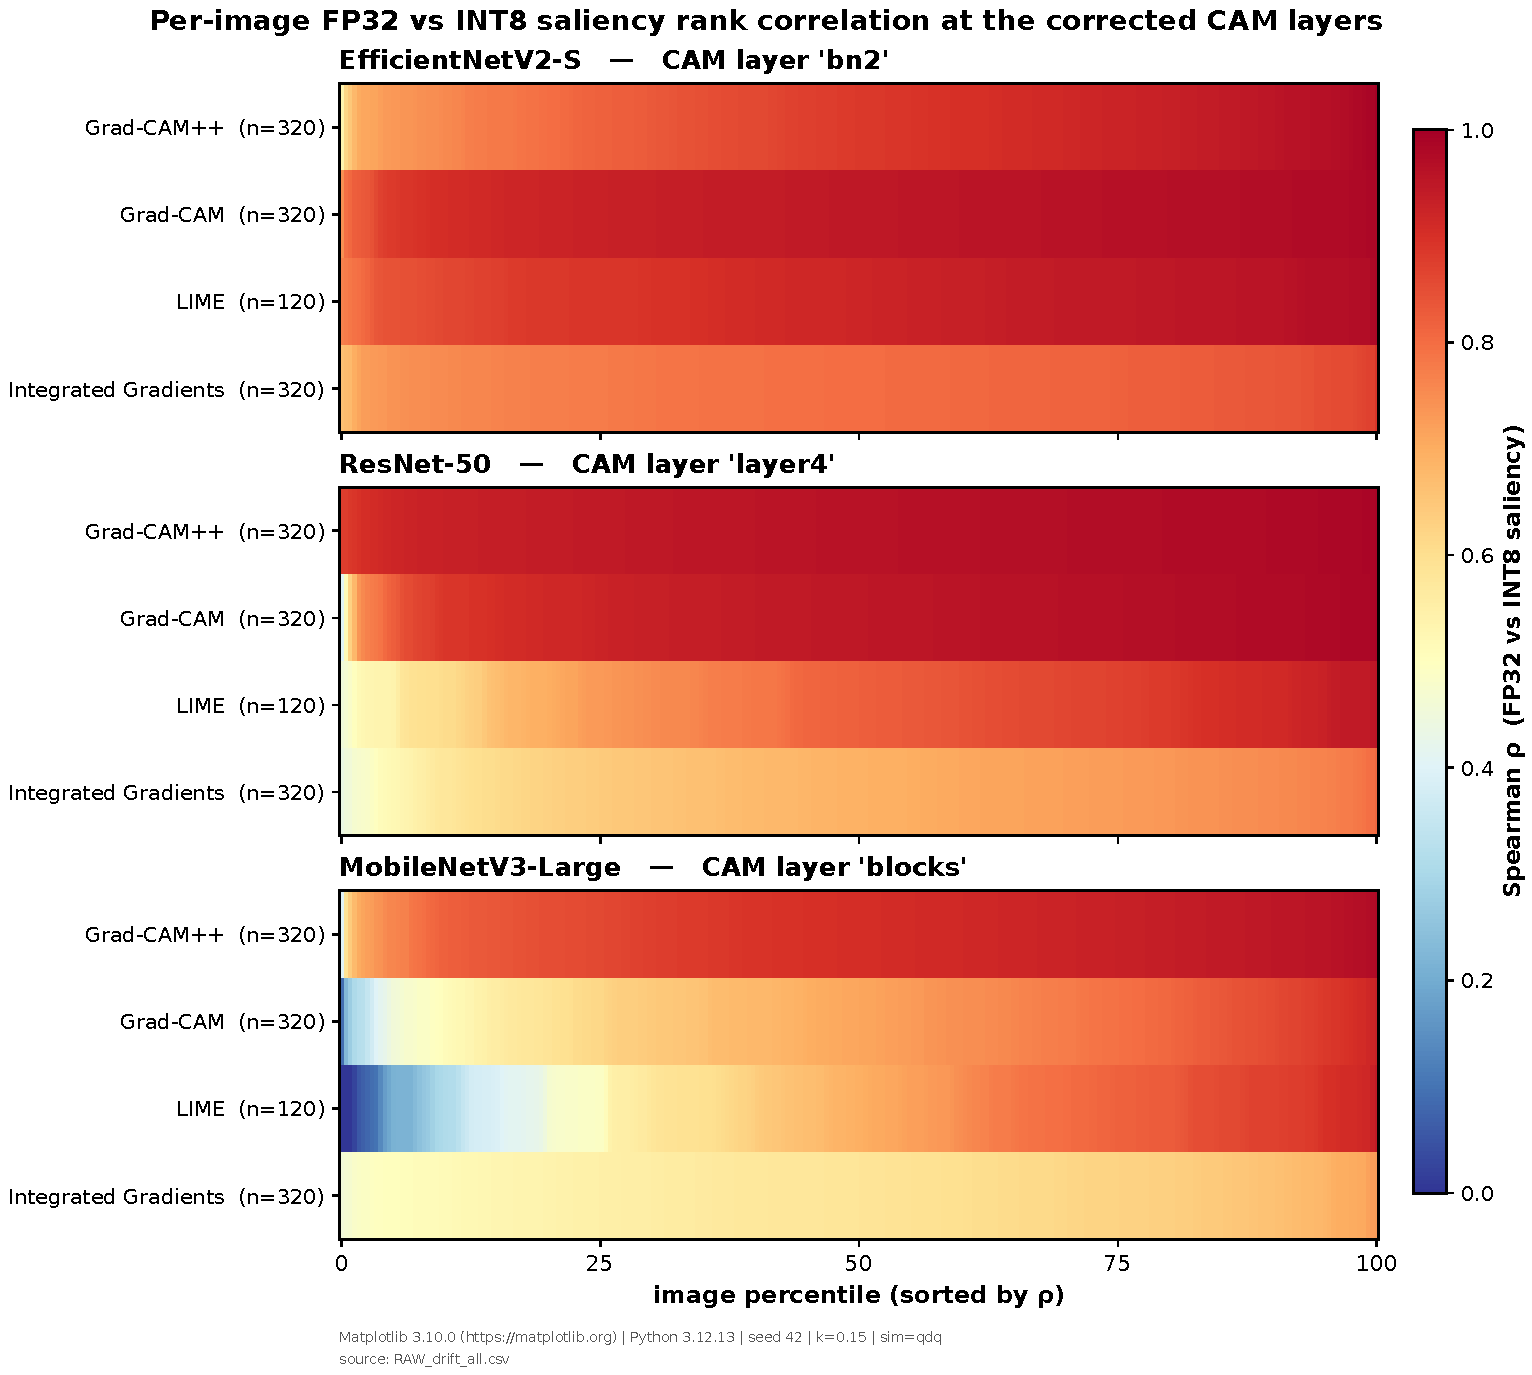
\includegraphics[width=0.92\textwidth]{figures/fig_spearman_grid.pdf}
\caption{Per-image FP32 versus INT8 saliency rank correlation at the resolved CAM target layers, $k = 0.15$. Each row is an architecture and each band within a row is an explanation method. Within a band the per-image Spearman $\rho$ values are sorted in ascending order and drawn left to right, so the horizontal axis is the image percentile and colour encodes $\rho$. This panel replaces the three per-image heatmaps of the original submission: no band is uniformly zero and no distribution is degenerate. Figure generated with Matplotlib 3.10.0 (\url{https://matplotlib.org}).}
\label{fig:spearman_grid}
\end{figure}

Figure~\ref{fig:spearman_grid} replaces the three separate per-image heatmaps of the original submission. Those heatmaps encoded $\rho$ for 20 individual images per architecture and, because the MobileNetV3-Large columns were uniformly zero under the degenerate target, invited exactly the misinterpretation corrected above. The replacement shows the full distribution over all 320 evaluation images per cell, and 120 for LIME.

\begin{figure}[!ht]
\centering
\begin{subfigure}[b]{0.49\textwidth}
    \centering
    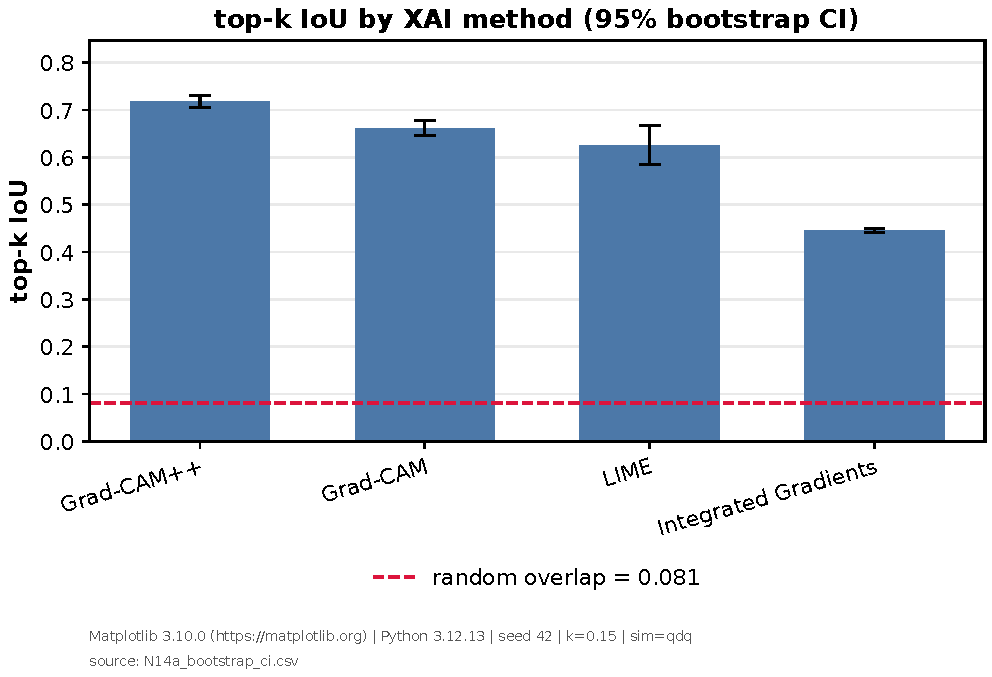
\includegraphics[width=\textwidth]{figures/fig_topk_iou_by_method_ci.pdf}
    \caption{Top-$k$ IoU}
\end{subfigure}\hfill
\begin{subfigure}[b]{0.49\textwidth}
    \centering
    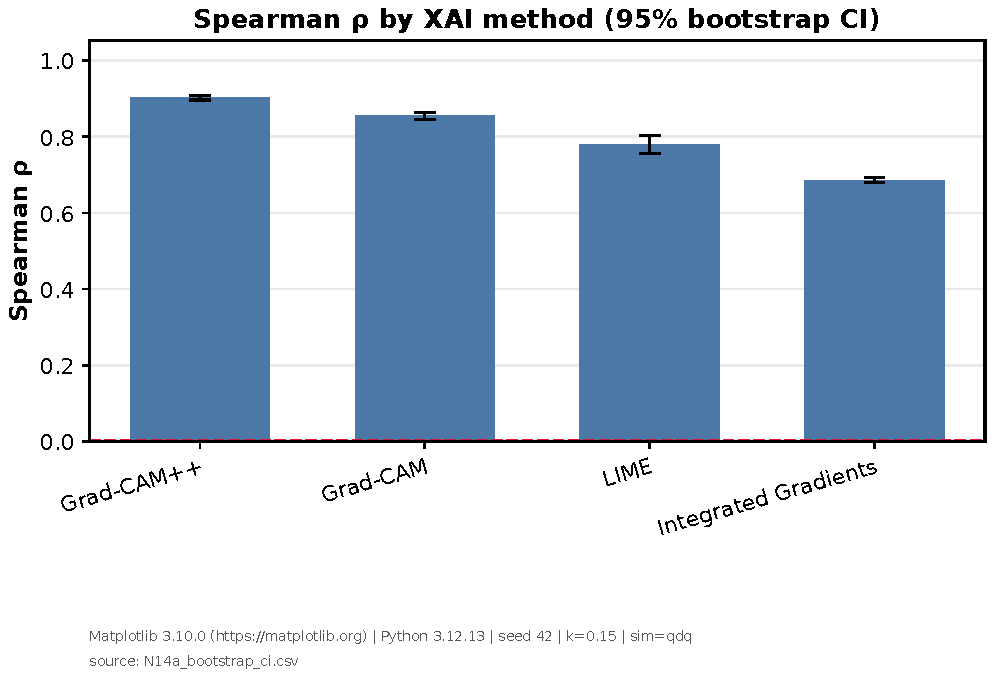
\includegraphics[width=\textwidth]{figures/fig_spearman_by_method_ci.pdf}
    \caption{Spearman $\rho$}
\end{subfigure}
\caption{Explanation drift by method and architecture with bootstrap $95\%$ confidence intervals. Dashed lines mark the random-overlap baseline. Every interval lies above the baseline. Figure generated with Matplotlib 3.10.0 (\url{https://matplotlib.org}).}
\label{fig:drift_comparison}
\end{figure}

\textbf{Method ranking.} Table~\ref{tab:method_ranking} aggregates across architectures. Grad-CAM++ is the best preserved method on every metric and also the most stable (coefficient of variation $0.176$), at $8.86\times$ chance. Integrated Gradients is the least preserved ($0.446$, $5.50\times$ chance). All six pairwise method comparisons remain significant after Holm correction, but one requires a caveat: Grad-CAM versus LIME has a mean paired difference of only $0.031$ with achieved power $0.601$, below the conventional $0.80$ threshold, and would need 576 paired LIME images rather than the 360 available. We therefore do not treat the Grad-CAM/LIME ordering as established.

\begin{table}[!ht]
\centering
\caption{Explanation method robustness aggregated across architectures at $k = 0.15$. CV is the coefficient of variation of top-$k$ IoU. The final column is the ratio of measured IoU to the random-overlap baseline of $0.081$.}
\label{tab:method_ranking}
\begin{tabular}{lc ccc cc}
\toprule
\textbf{Method} & \textbf{$n$} & \textbf{Top-$k$ IoU} & \textbf{Top-$k$ Dice} & \textbf{Spearman $\rho$} & \textbf{IoU CV} & \textbf{vs.\ chance} \\
\midrule
Grad-CAM++ & 960 & 0.718 & 0.829 & 0.903 & 0.176 & 8.86$\times$ \\
Grad-CAM & 960 & 0.662 & 0.775 & 0.855 & 0.310 & 8.16$\times$ \\
LIME & 360 & 0.625 & 0.732 & 0.780 & 0.427 & 7.71$\times$ \\
Int.\ Gradients & 960 & 0.446 & 0.611 & 0.686 & 0.204 & 5.50$\times$ \\
\bottomrule
\end{tabular}
\end{table}

\subsection*{Sensitivity to the top-$k$ threshold}

Table~\ref{tab:k_sweep} recomputes drift over $k \in [0.05, 0.30]$. Absolute IoU rises with $k$ for the three gradient methods, but so does the random baseline, and the ratio to chance is approximately flat; LIME is the exception, declining slightly from $0.657$ to $0.635$. Spearman $\rho$ is invariant to $k$ by construction, since it is computed on continuous maps before binarisation.

\begin{table}[!ht]
\centering
\caption{Top-$k$ IoU as a function of $k$ (resolved targets, aggregated across architectures), with the analytic random-overlap baseline for reference. The primary operating point is $k = 0.15$.}
\label{tab:k_sweep}
\begin{tabular}{lcccccc}
\toprule
\textbf{Method} & 0.05 & 0.10 & 0.15 & 0.20 & 0.25 & 0.30 \\
\midrule
Grad-CAM & 0.568 & 0.630 & 0.662 & 0.682 & 0.698 & 0.712 \\
Grad-CAM++ & 0.632 & 0.690 & 0.718 & 0.736 & 0.749 & 0.758 \\
Int.\ Gradients & 0.391 & 0.420 & 0.446 & 0.470 & 0.494 & 0.517 \\
LIME & 0.657 & 0.643 & 0.625 & 0.625 & 0.632 & 0.635 \\
\midrule
Random baseline & 0.026 & 0.053 & 0.081 & 0.111 & 0.143 & 0.176 \\
\bottomrule
\end{tabular}
\end{table}

Table~\ref{tab:rank_stability} reports a finding that qualifies our method-level conclusions and that we did not anticipate. The \emph{architecture} ranking is stable across $k$ (Kendall $\tau = 1.0$ at five of six thresholds). The \emph{method} ranking is not. At $k = 0.05$ LIME ranks first; from $k = 0.15$ onward it ranks third, and $\tau$ against the $k = 0.05$ ordering falls to $0.333$. The instability is confined to the LIME/Grad-CAM/Grad-CAM++ group, which Table~\ref{tab:method_ranking} already shows to be closely spaced and, for Grad-CAM versus LIME, underpowered. Integrated Gradients ranks last at every threshold. We therefore restrict our method-level claim to what survives the sweep: Integrated Gradients is robustly the least preserved method, and the ordering among the remaining three is threshold-dependent and should not be treated as a general recommendation.

\begin{table}[!ht]
\centering
\scriptsize
\caption{Stability of the explanation-method ranking across top-$k$ thresholds. Kendall $\tau$ is computed against the ordering at $k = 0.05$. The ranking is not stable, which bounds the strength of method-level recommendations.}
\label{tab:rank_stability}
\setlength{\tabcolsep}{4pt}
\begin{tabular}{lll}
\toprule
\textbf{$k$} & \textbf{Ranking by top-$k$ IoU} & \textbf{Kendall $\tau$ vs.\ $k=0.05$} \\
\midrule
0.05 & LIME $\succ$ Grad-CAM++ $\succ$ Grad-CAM $\succ$ Int.\ Gradients & 1.000 \\
0.10 & Grad-CAM++ $\succ$ LIME $\succ$ Grad-CAM $\succ$ Int.\ Gradients & 0.667 \\
0.15 & Grad-CAM++ $\succ$ Grad-CAM $\succ$ LIME $\succ$ Int.\ Gradients & 0.333 \\
0.20 & Grad-CAM++ $\succ$ Grad-CAM $\succ$ LIME $\succ$ Int.\ Gradients & 0.333 \\
0.25 & Grad-CAM++ $\succ$ Grad-CAM $\succ$ LIME $\succ$ Int.\ Gradients & 0.333 \\
0.30 & Grad-CAM++ $\succ$ Grad-CAM $\succ$ LIME $\succ$ Int.\ Gradients & 0.333 \\
\bottomrule
\end{tabular}
\end{table}

\begin{figure}[!ht]
\centering
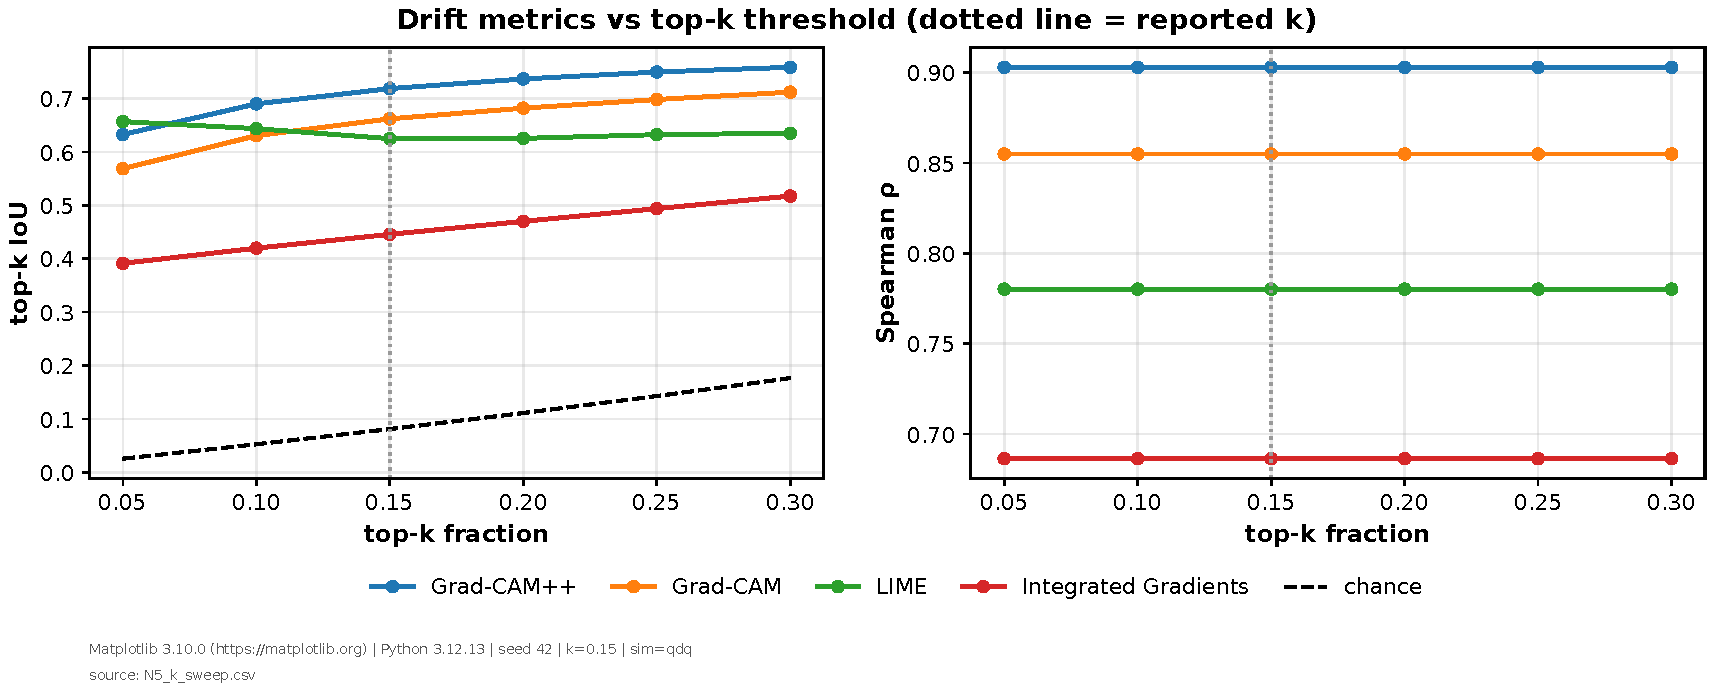
\includegraphics[width=0.80\textwidth]{figures/fig_k_sweep.pdf}
\caption{Top-$k$ IoU as a function of the threshold $k$, by explanation method, with the analytic random-overlap baseline $k/(2-k)$ shown dashed. Figure generated with Matplotlib 3.10.0 (\url{https://matplotlib.org}).}
\label{fig:k_sweep}
\end{figure}

\subsection*{Replication, sanity checks, and mixed precision}

Seed replication at 42, 1337, and 2024 gives standard deviations of $0.002$--$0.009$ in top-$k$ IoU across all nine architecture--method cells, one to two orders of magnitude smaller than the between-method differences being interpreted, so the reported ordering is not a seed artefact.

The cascading parameter-randomisation check behaves as required: rank correlation between saliency from the trained model and from progressively randomised models stays within $[-0.166, 0.215]$ at all randomisation fractions, indicating the attribution pipeline is sensitive to learned weights rather than to architecture alone. This check used 16 images per cell and is reported as a qualitative sanity result, not a powered comparison.

Mixed precision resolves most of the residual drift and provides the most actionable deployment recommendation in this study. Retaining only the CAM target stage in FP32 while quantizing the rest of the network raises top-$k$ IoU from $0.582$ to $0.841$ for MobileNetV3-Large and from $0.702$ to $0.823$ for EfficientNetV2-S, with $\rho$ reaching $0.971$ and $0.967$ (Table~\ref{tab:mixed_precision}). ResNet-50, which already preserves attribution well, changes little. Since the CAM target stage is a small fraction of total parameters, this recovers explanation fidelity at modest cost in compression.

\begin{table}[!ht]
\centering
\scriptsize
\caption{Mixed-precision intervention. ``All INT8'' quantizes the whole network; ``CAM stage FP32'' retains the resolved target stage in full precision. Collapse rate is $0.000$ in all conditions. The ``All INT8'' columns are averaged over Grad-CAM and Grad-CAM++ at the resolved target layer and therefore equal the mean of the two CAM rows for the corresponding architecture in Table~\ref{tab:drift_main}: $(0.736+0.667)/2 = 0.702$ for EfficientNetV2-S, $(0.783+0.790)/2 = 0.786$ for ResNet-50, and $(0.467+0.698)/2 = 0.582$ for MobileNetV3-Large. Integrated Gradients and LIME are excluded because the intervention modifies only the CAM target stage.}
\label{tab:mixed_precision}
\setlength{\tabcolsep}{5pt}
\begin{tabular}{ll cc cc}
\toprule
 & & \multicolumn{2}{c}{\textbf{Top-$k$ IoU}} & \multicolumn{2}{c}{\textbf{Spearman $\rho$}} \\
\cmidrule(lr){3-4} \cmidrule(lr){5-6}
\textbf{Architecture} & \textbf{FP32 stage} & \textbf{All INT8} & \textbf{CAM stage FP32} & \textbf{All INT8} & \textbf{CAM stage FP32} \\
\midrule
EfficientNetV2-S  & \texttt{bn2}   & 0.702 & \textbf{0.823} & 0.903 & \textbf{0.967} \\
ResNet-50         & \texttt{layer4} & 0.786 & 0.791 & 0.943 & 0.946 \\
MobileNetV3-Large & \texttt{blocks} & 0.582 & \textbf{0.841} & 0.790 & \textbf{0.971} \\
\bottomrule
\end{tabular}
\end{table}

\subsection*{Explanation-aware QAT is architecture-dependent}

Table~\ref{tab:lambda_sweep} reports the dose--response over the consistency weight $\lambda$, including the $\lambda = 0$ control that is identical to standard QAT.

\begin{table}[!ht]
\centering
\scriptsize
\caption{Top-$k$ IoU as a function of the CAM-consistency weight $\lambda$. The $\lambda = 0$ column is the standard-QAT control; any benefit attributed to explanation-aware QAT must exceed it.}
\label{tab:lambda_sweep}
\setlength{\tabcolsep}{5pt}
\begin{tabular}{ll ccccc}
\toprule
\textbf{Architecture} & \textbf{Method} & $\lambda=0$ & $\lambda=0.1$ & $\lambda=0.5$ & $\lambda=1$ & $\lambda=2$ \\
\midrule
\multirow{3}{*}{EfficientNetV2-S}
 & Grad-CAM & 0.643 & 0.661 & 0.673 & 0.690 & 0.705 \\
 & Grad-CAM++ & 0.479 & 0.503 & 0.550 & 0.557 & 0.587 \\
 & Int.\ Gradients & 0.397 & 0.402 & 0.407 & 0.421 & 0.429 \\
\midrule
\multirow{3}{*}{ResNet-50}
 & Grad-CAM & 0.778 & 0.779 & 0.779 & 0.777 & 0.788 \\
 & Grad-CAM++ & 0.774 & 0.778 & 0.782 & 0.777 & 0.786 \\
 & Int.\ Gradients & 0.402 & 0.411 & 0.409 & 0.412 & 0.406 \\
\midrule
\multirow{3}{*}{MobileNetV3-L}
 & Grad-CAM & 0.515 & 0.526 & 0.542 & 0.554 & 0.578 \\
 & Grad-CAM++ & 0.724 & 0.722 & 0.732 & 0.730 & 0.732 \\
 & Int.\ Gradients & 0.394 & 0.399 & 0.399 & 0.403 & 0.409 \\
\bottomrule
\end{tabular}
\end{table}

Table~\ref{tab:mitigation} compares baseline PTQ drift with $\lambda = 0.5$ QAT, with Holm-corrected paired tests.

\begin{table}[!ht]
\centering
\scriptsize
\caption{QAT mitigation at $\lambda = 0.5$ versus PTQ baseline, replicated over three seeds. $\Delta$ is relative change; $p$ values are Holm-corrected paired tests on 320 image pairs.}
\label{tab:mitigation}
\setlength{\tabcolsep}{4pt}
\begin{tabular}{ll ccc ccc cc}
\toprule
 & & \multicolumn{3}{c}{\textbf{Top-$k$ IoU}} & \multicolumn{3}{c}{\textbf{Spearman $\rho$}} & & \\
\cmidrule(lr){3-5} \cmidrule(lr){6-8}
\textbf{Architecture} & \textbf{Method} & \textbf{PTQ} & \textbf{QAT} & \textbf{$\Delta\%$} & \textbf{PTQ} & \textbf{QAT} & \textbf{$\Delta\%$} & \textbf{$p_{\text{Holm}}$} & \textbf{Sig.} \\
\midrule
\multirow{3}{*}{EfficientNetV2-S}
 & Grad-CAM & 0.736 & 0.673 & $-8.5$ & 0.940 & 0.897 & $-4.6$ & 0.0000 & yes \\
 & Grad-CAM++ & 0.667 & 0.550 & $-17.5$ & 0.866 & 0.738 & $-14.8$ & 0.0000 & yes \\
 & Int.\ Gradients & 0.550 & 0.407 & $-26.0$ & 0.797 & 0.659 & $-17.2$ & 0.0000 & yes \\
\midrule
\multirow{3}{*}{ResNet-50}
 & Grad-CAM & 0.783 & 0.779 & $-0.5$ & 0.931 & 0.931 & $-0.0$ & 0.8772 & \textbf{no} \\
 & Grad-CAM++ & 0.790 & 0.782 & $-1.0$ & 0.955 & 0.951 & $-0.5$ & 0.8772 & \textbf{no} \\
 & Int.\ Gradients & 0.420 & 0.409 & $-2.6$ & 0.676 & 0.664 & $-1.7$ & 0.0000 & yes \\
\midrule
\multirow{3}{*}{MobileNetV3-L}
 & Grad-CAM & 0.467 & 0.542 & $+16.3$ & 0.693 & 0.782 & $+12.8$ & 0.0000 & yes \\
 & Grad-CAM++ & 0.698 & 0.732 & $+4.8$ & 0.887 & 0.925 & $+4.3$ & 0.0000 & yes \\
 & Int.\ Gradients & 0.366 & 0.399 & $+9.2$ & 0.587 & 0.628 & $+7.1$ & 0.0000 & yes \\
\bottomrule
\end{tabular}
\end{table}

The effect is directional by architecture, and in two of three cases it is not beneficial. MobileNetV3-Large improves on all three methods (top-$k$ IoU $+16.3\%$, $+4.8\%$, $+9.2\%$; all $p_{\text{Holm}} < 0.001$). ResNet-50 is essentially unchanged, and its two CAM comparisons are not significant ($p_{\text{Holm}} = 0.877$). EfficientNetV2-S is significantly \emph{degraded} on all three methods ($-8.5\%$, $-17.5\%$, $-26.0\%$). These comparisons are taken against the PTQ baseline and therefore measure quantization-aware training and the consistency term together. Table~\ref{tab:qat_control} separates the two against a $\lambda = 0$ control and shows that the architecture dependence originates in quantization-aware training itself, not in the consistency term. Explanation-aware QAT is consequently a targeted repair for the architecture whose attribution was most disturbed, and a net harm where plain quantization-aware training is itself harmful.

We also withdraw the specific headline of the original submission. The previously reported ``up to $49.2\%$ improvement in Spearman correlation'' was a relative change computed on a baseline of $\rho = -0.120$ rising to $\rho = -0.061$. Both values are negative; the explanation was anti-correlated before and after. Reporting that as a $49.2\%$ improvement was misleading, and it does not appear in this revision.

Table~\ref{tab:post_qat} reports post-QAT classification performance, which the original submission did not measure. Explanation-aware QAT does not cost accuracy: at $\lambda = 0.5$ all three architectures stay within $0.5$ percentage points of their FP32 macro-F1, and every QAT variant improves FP32--INT8 prediction agreement over plain PTQ. The concern that the consistency term trades accuracy for explanation stability is not supported.

\begin{table}[!ht]
\centering
\scriptsize
\caption{Classification performance after quantization and after explanation-aware QAT, on the validation split at seed 42. Agreement is top-1 agreement with the FP32 model.}
\label{tab:post_qat}
\setlength{\tabcolsep}{5pt}
\begin{tabular}{ll cccc}
\toprule
\textbf{Architecture} & \textbf{Stage} & \textbf{Accuracy} & \textbf{Macro-F1} & \textbf{Balanced acc.} & \textbf{Agreement} \\
\midrule
\multirow{7}{*}{EfficientNetV2-S}
 & FP32 & 0.9793 & 0.9796 & 0.9767 & 1.0000 \\
 & PTQ-INT8 & 0.9755 & 0.9752 & 0.9717 & 0.9914 \\
 & QAT-INT8 ($\lambda=0$) & 0.9731 & 0.9736 & 0.9746 & 0.9803 \\
 & QAT-INT8 ($\lambda=0.1$) & 0.9755 & 0.9756 & 0.9763 & 0.9808 \\
 & QAT-INT8 ($\lambda=0.5$) & 0.9745 & 0.9741 & 0.9759 & 0.9803 \\
 & QAT-INT8 ($\lambda=1$) & 0.9755 & 0.9765 & 0.9760 & 0.9813 \\
 & QAT-INT8 ($\lambda=2$) & 0.9741 & 0.9752 & 0.9752 & 0.9808 \\
\midrule
\multirow{7}{*}{ResNet-50}
 & FP32 & 0.9745 & 0.9709 & 0.9688 & 1.0000 \\
 & PTQ-INT8 & 0.9500 & 0.9464 & 0.9442 & 0.9654 \\
 & QAT-INT8 ($\lambda=0$) & 0.9693 & 0.9653 & 0.9641 & 0.9832 \\
 & QAT-INT8 ($\lambda=0.1$) & 0.9645 & 0.9589 & 0.9588 & 0.9789 \\
 & QAT-INT8 ($\lambda=0.5$) & 0.9625 & 0.9583 & 0.9577 & 0.9750 \\
 & QAT-INT8 ($\lambda=1$) & 0.9669 & 0.9627 & 0.9640 & 0.9760 \\
 & QAT-INT8 ($\lambda=2$) & 0.9640 & 0.9586 & 0.9588 & 0.9803 \\
\midrule
\multirow{7}{*}{MobileNetV3-L}
 & FP32 & 0.9750 & 0.9732 & 0.9696 & 1.0000 \\
 & PTQ-INT8 & 0.9577 & 0.9535 & 0.9469 & 0.9707 \\
 & QAT-INT8 ($\lambda=0$) & 0.9707 & 0.9711 & 0.9714 & 0.9765 \\
 & QAT-INT8 ($\lambda=0.1$) & 0.9741 & 0.9734 & 0.9726 & 0.9808 \\
 & QAT-INT8 ($\lambda=0.5$) & 0.9712 & 0.9723 & 0.9719 & 0.9784 \\
 & QAT-INT8 ($\lambda=1$) & 0.9731 & 0.9737 & 0.9735 & 0.9803 \\
 & QAT-INT8 ($\lambda=2$) & 0.9726 & 0.9740 & 0.9737 & 0.9808 \\
\bottomrule
\end{tabular}
\end{table}

\begin{figure}[!ht]
\centering
\begin{subfigure}[b]{0.49\textwidth}
    \centering
    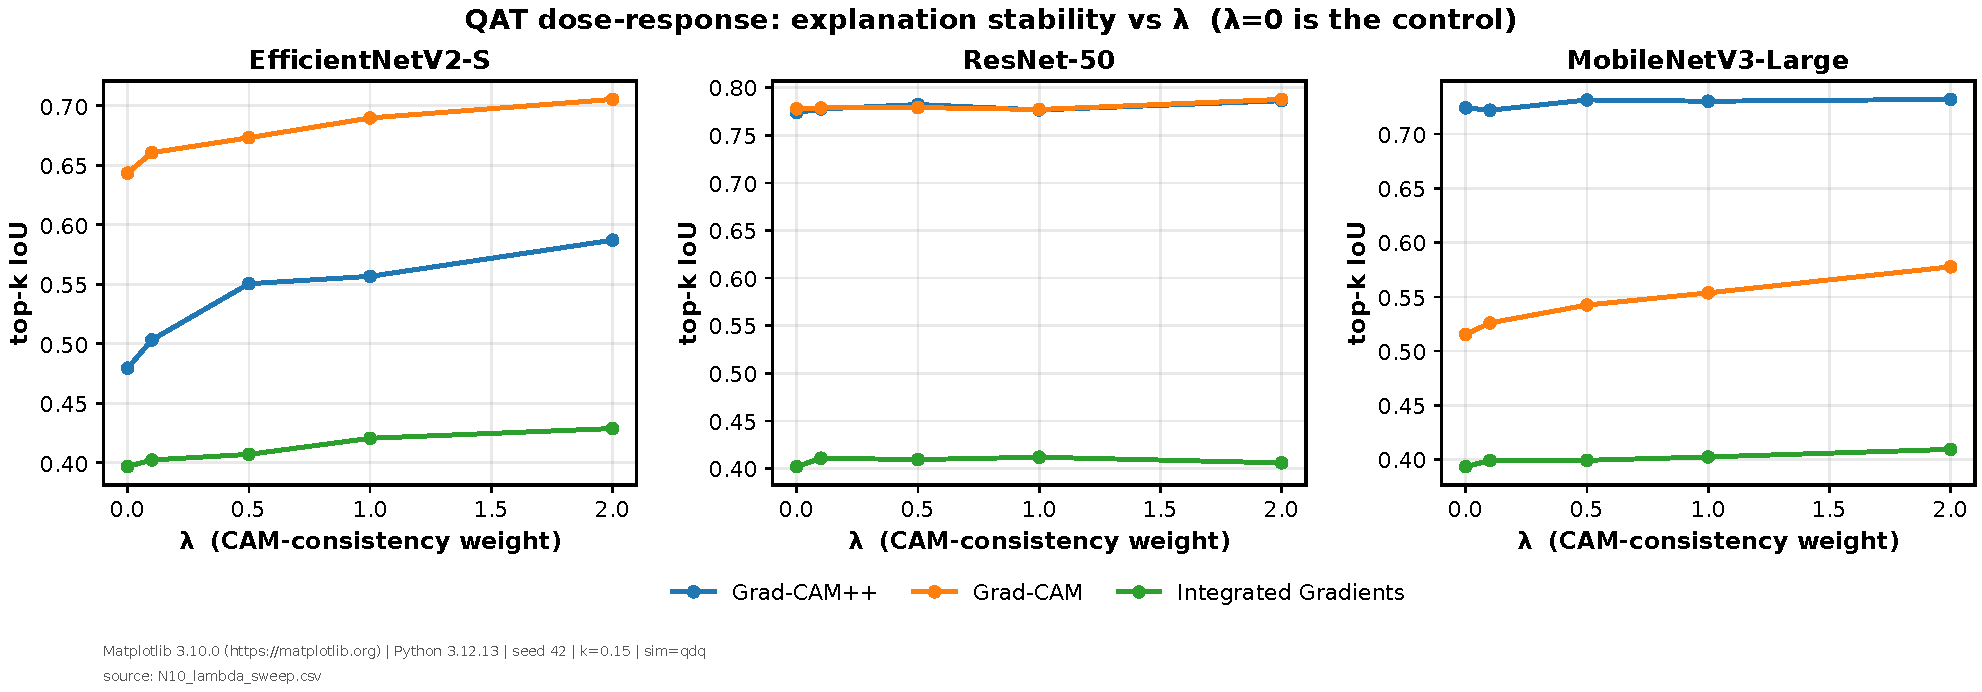
\includegraphics[width=\textwidth]{figures/fig_lambda_sweep.pdf}
    \caption{Drift versus $\lambda$}
\end{subfigure}\hfill
\begin{subfigure}[b]{0.49\textwidth}
    \centering
    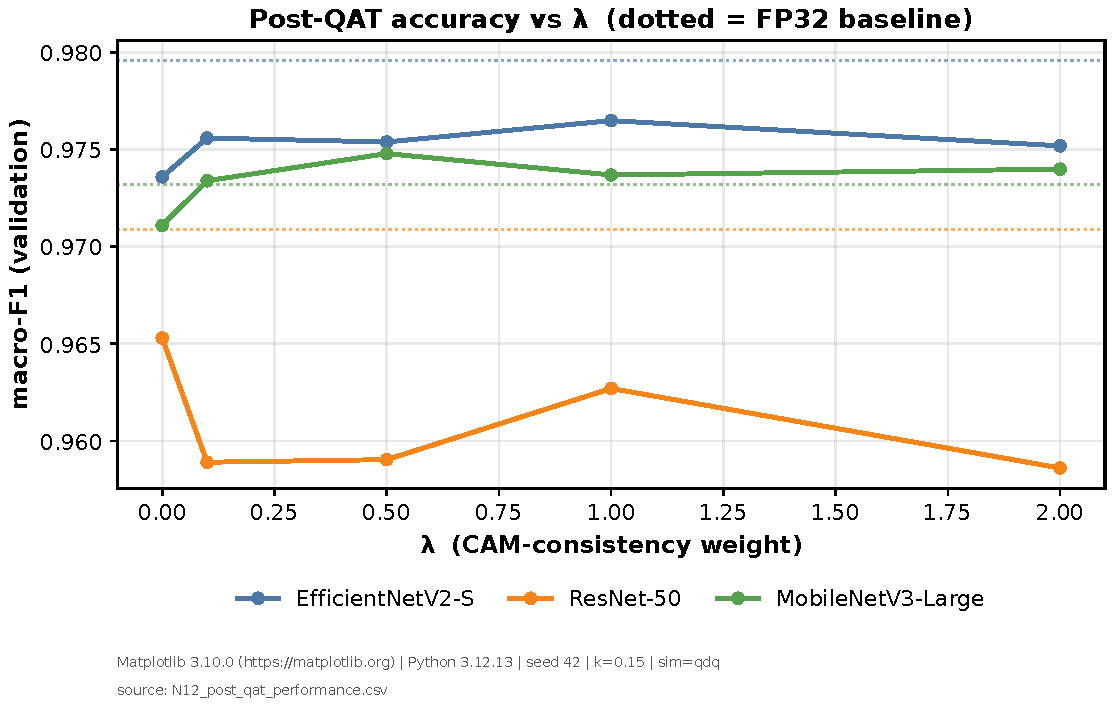
\includegraphics[width=\textwidth]{figures/fig_accuracy_vs_lambda.pdf}
    \caption{Accuracy versus $\lambda$}
\end{subfigure}
\caption{Dose--response for the CAM-consistency weight $\lambda$. The $\lambda = 0$ point is the standard-QAT control. Figures generated with Matplotlib 3.10.0 (\url{https://matplotlib.org}).}
\label{fig:lambda_sweep}
\end{figure}

\subsection*{Class imbalance, per-class drift, and lesion morphology}

We tested directly whether class frequency predicts drift severity. Across the 10 classes the Spearman correlation between class frequency and mean top-$k$ IoU is $-0.358$ (MobileNetV3-Large, $p = 0.310$), $-0.261$ (ResNet-50, $p = 0.467$), and $-0.333$ (EfficientNetV2-S, $p = 0.347$); against mean $\rho$ the correlations are $-0.430$, $-0.491$, and $-0.261$ (all $p > 0.14$). No association reaches significance in any architecture on either metric, and with 10 classes the test is underpowered for the moderate negative correlations observed. The honest conclusion is that we cannot detect a class-imbalance effect on explanation drift at this sample size, and we no longer claim one.

For the same reason we withdraw the lesion-morphology explanation offered in the original submission, which argued that diseases with localised high-contrast lesions retain saliency better than those with diffuse symptoms. That claim rested on per-class means computed from two images per class, was not tested against a null, and is not supported once class-level drift is examined against class frequency. Per-class drift metrics are retained in the supplementary material and are labelled \emph{exploratory}: with 32 images per class they are descriptive, not inferential, and no mechanism is attributed to them.

\subsection*{Faithfulness: similarity is not quality}

A preserved explanation is not necessarily a correct one, and drift metrics alone cannot distinguish the two. We therefore evaluated faithfulness directly and, separately, against expert annotations.

Deletion and insertion curves, confidence drop, infidelity, and maximum sensitivity were computed for FP32 and INT8 models (Table~\ref{tab:faithfulness}). The pattern is consistent across architectures: aggregate faithfulness changes only modestly under quantization, but maximum sensitivity, which measures how much an explanation changes under small input perturbations, worsens markedly in every case, for example $0.096 \rightarrow 0.352$ for ResNet-50 Grad-CAM and $0.337 \rightarrow 0.571$ for MobileNetV3-Large. Confidence drop falls under quantization for every architecture ($0.742 \rightarrow 0.689$, $0.776 \rightarrow 0.738$, and $0.766 \rightarrow 0.648$): masking the region an INT8 explanation identifies as salient perturbs the prediction slightly less than for FP32, consistent with the small reductions in insertion AUC. Quantized explanations are thus similar on average but less stable locally, a degradation invisible to similarity metrics alone.

\begin{table}[!ht]
\centering
\scriptsize
\caption{Faithfulness of FP32 and INT8 explanations ($n = 250$ images; infidelity and sensitivity on 64). Lower deletion AUC, higher insertion AUC, lower infidelity and lower sensitivity indicate better explanations. Conf.\ drop is the mean relative fall in the predicted-class probability when the top-$k$ salient region is masked, so a larger value indicates a more faithful explanation.}
\label{tab:faithfulness}
\setlength{\tabcolsep}{4pt}
\begin{tabular}{llccccc}
\toprule
\textbf{Architecture} & \textbf{Model} & \textbf{Deletion AUC} & \textbf{Insertion AUC} & \textbf{Conf.\ drop} & \textbf{Infidelity} & \textbf{Sensitivity$_{\max}$} \\
\midrule
\multirow{2}{*}{EfficientNetV2-S}  & FP32 & 0.288 & 0.575 & 0.742 & 59.40 & 0.172 \\
                                   & INT8 & 0.270 & 0.534 & 0.689 & 55.04 & 0.310 \\
\midrule
\multirow{2}{*}{ResNet-50}         & FP32 & 0.249 & 0.713 & 0.776 & 45.91 & 0.096 \\
                                   & INT8 & 0.232 & 0.676 & 0.738 & 45.81 & 0.352 \\
\midrule
\multirow{2}{*}{MobileNetV3-Large} & FP32 & 0.174 & 0.266 & 0.766 & 47.68 & 0.337 \\
                                   & INT8 & 0.171 & 0.277 & 0.648 & 39.85 & 0.571 \\
\bottomrule
\end{tabular}
\end{table}

Because the Paddy dataset has no lesion masks, we added an external ground-truth localisation test on the SIIM-ACR Pneumothorax dataset, which provides expert pixel-level annotations. A binary classifier was fine-tuned from the same backbone, quantized identically, and Grad-CAM overlap with expert masks was measured on 87 annotated positive cases. The result is a negative one and we report it as such: mean IoU against expert masks is $0.0066$ for FP32 and $0.0106$ for INT8, against a chance level of $0.0073$; the pointing-game score is $0.000$ for FP32 and $0.011$ for INT8; and a paired Wilcoxon test finds no difference between them ($W = 122$, $z = -0.49$, $p = 0.627$, with 64 of 87 cases exactly tied). Neither model localises the annotated pathology better than chance. A large part of the explanation is structural: the annotated lesions occupy a mean $1.43\%$ of image area, whereas a single cell of the $7 \times 7$ CAM grid covers $2.04\%$, so the CAM resolution is coarser than the target. We draw the conservative conclusion that explanation \emph{similarity} between FP32 and INT8, which is high, must not be read as explanation \emph{quality}, which we could not establish for either precision.


% ============================================================================
% DISCUSSION
% ============================================================================

\subsection*{Simulated versus deployed INT8: agreement, logits, and intermediate features}

Because every gradient-based drift metric in this paper is computed on the PyTorch fake-quantized model rather than on the integer ONNX Runtime graph, the equivalence of the two is a load-bearing assumption, and we characterise it directly (Table~\ref{tab:equivalence}) rather than deferring it to the released code.

On the full validation split of 2{,}082 images, top-1 agreement between the FP32 model and the fake-quantized INT8 model is $0.9914$ for EfficientNetV2-S, $0.9654$ for ResNet-50, and $0.9707$ for MobileNetV3-Large. Agreement on the 320-image explanation subset is within $0.7$ percentage points of the full-split value for all three architectures. The same subset-to-split comparison for the deployed graph under percentile calibration gives differences of $+1.1$, $-0.7$, and $+2.4$ percentage points; the only case in which the subset over-estimates agreement is ResNet-50, and it does so by $0.7$ points. The evaluation subset is therefore a representative, and for two of three architectures a slightly conservative, sample of the split.

Agreement alone can conceal changes in decision margin, so we also report logit-level differences. The mean absolute logit difference between FP32 and fake-quantized INT8 is $0.256$, $0.329$, and $0.517$ for the three architectures, with maximum absolute differences of $1.65$, $3.03$, and $3.26$ and logit cosine similarity of $0.978$, $0.961$, and $0.909$. This ordering matches the drift ordering reported above: MobileNetV3-Large is both the least faithfully simulated and the least explanation-stable model.

Finally, we quantify intermediate-feature similarity using linear centred kernel alignment (CKA) between FP32 and INT8 activations. At an early layer (\texttt{bn1}) CKA is at least $0.999$ for all three architectures, confirming that quantization error is negligible near the input and accumulates with depth. At the resolved CAM target layer, CKA is $0.913$, $0.777$, and $0.885$. The contrast with the legacy configuration is informative: at ResNet-50 \texttt{layer4}, CKA is $0.777$ under the resolved configuration but only $0.272$ under the legacy configuration, providing independent evidence that the original analysis was reading from a representation degraded by the extraction path rather than by quantization.

Because agreement with the fake-quantized model alone does not establish that the \emph{deployed} graph behaves the same way, we also evaluated the exported ONNX Runtime graphs on all $2{,}082$ validation images under each of the three calibrators. Under the deployed percentile configuration, top-1 agreement with FP32 is $0.9270$ for EfficientNetV2-S, $0.9707$ for ResNet-50, and $0.9145$ for MobileNetV3-Large, with mean absolute logit differences of $0.579$, $0.288$, and $0.615$ and logit cosine similarity of $0.855$, $0.963$, and $0.835$. Deployed INT8 top-1 accuracy on the full split is $0.9174$, $0.9568$, and $0.9015$, against FP32 accuracies of $0.9793$, $0.9745$, and $0.9750$.

Two consequences follow, and we state both plainly. First, for EfficientNetV2-S and MobileNetV3-Large the fake-quantized model is a closer match to FP32 than the deployed graph is ($0.9914$ and $0.9707$ agreement versus $0.9270$ and $0.9145$), so the simulation is mildly optimistic and the drift magnitudes reported in this paper should be read as a lower bound on what the deployed integer graph would exhibit; ResNet-50 is the exception, where the two realisations track FP32 to within $0.005$. Second, because both realisations are compared against the same FP32 reference, the union bound forces them to agree with each other on at least $91.8\%$, $93.6\%$, and $88.5\%$ of the validation split. That supports interchangeability for prediction but does not prove it for explanations: the integer runtime exposes no gradients and no intermediate activations, so a direct saliency comparison between the two engines is not possible with any gradient-based method, and we record this as a limitation rather than a resolved question.

\begin{table}[htbp]
\centering
\caption{Equivalence between the PyTorch fake-quantized model used for explanation analysis and the deployed ONNX Runtime INT8 graph. For the ONNX Runtime rows, top-1 agreement and all logit statistics are computed on the \emph{full} validation split ($n=2{,}082$); the $n{=}320$ column repeats the agreement obtained on the explanation evaluation subset so that the two can be compared directly. For the fake-quantized rows, agreement is reported on both the full split and the subset, while logit statistics and CKA are computed on the 320-image subset on which all explanation analyses are performed. Logit MAE and Max are absolute differences in logit units relative to the corresponding FP32 engine, and Cosine is the FP32--INT8 logit cosine similarity. CKA is linear centred kernel alignment at an early layer (\texttt{bn1}) and at the resolved CAM target layer; the ONNX Runtime graph exposes no intermediate activations, so CKA is undefined for those rows. Percentile calibration is the deployed configuration; entropy and MinMax are reported as calibration controls, MinMax being the documented negative control of Table~\ref{tab:calib_ablation}.}
\label{tab:equivalence}
\small
\begin{tabular}{llcccccc}
\toprule
 & & \multicolumn{2}{c}{\textbf{Top-1 agreement}} & \multicolumn{3}{c}{\textbf{Logit difference vs.\ FP32}} & \textbf{CKA} \\
\cmidrule(lr){3-4}\cmidrule(lr){5-7}\cmidrule(lr){8-8}
\textbf{Architecture} & \textbf{Engine} & $n{=}2{,}082$ & $n{=}320$ & MAE & Max & Cosine & \texttt{bn1} / CAM \\
\midrule
\multirow{4}{*}{EfficientNetV2-S}
  & Fake-quant (QDQ) & 0.9914 & 0.9844 & 0.256 & 1.653 & 0.978 & 0.999 / 0.913 \\
  & ONNX Runtime (Percentile) & 0.9270 & 0.9156 & 0.579 & 4.608 & 0.855 & --- \\
  & ONNX Runtime (Entropy) & 0.7498 & 0.7375 & 0.818 & 6.604 & 0.605 & --- \\
  & ONNX Runtime (MinMax) & 0.6441 & 0.6344 & 1.091 & 7.042 & 0.417 & --- \\
\midrule
\multirow{4}{*}{ResNet-50}
  & Fake-quant (QDQ) & 0.9654 & 0.9656 & 0.329 & 3.028 & 0.961 & 1.000 / 0.777 \\
  & ONNX Runtime (Percentile) & 0.9707 & 0.9781 & 0.288 & 4.392 & 0.963 & --- \\
  & ONNX Runtime (Entropy) & 0.9669 & 0.9656 & 0.329 & 4.113 & 0.957 & --- \\
  & ONNX Runtime (MinMax) & 0.9107 & 0.9000 & 0.526 & 5.141 & 0.886 & --- \\
\midrule
\multirow{4}{*}{MobileNetV3-Large}
  & Fake-quant (QDQ) & 0.9707 & 0.9688 & 0.517 & 3.261 & 0.909 & 1.000 / 0.885 \\
  & ONNX Runtime (Percentile) & 0.9145 & 0.8906 & 0.615 & 5.621 & 0.835 & --- \\
  & ONNX Runtime (Entropy) & 0.8132 & 0.7688 & 0.803 & 6.317 & 0.711 & --- \\
  & ONNX Runtime (MinMax) & 0.6412 & 0.5469 & 0.946 & 7.463 & 0.563 & --- \\
\bottomrule
\end{tabular}
\end{table}

\subsection*{A direct test of the per-channel collapse mechanism}

The mechanism proposed in the original submission, that depthwise-separable convolutions are intrinsically more vulnerable to per-channel range compression, is testable, and we tested it rather than merely withdrawing it. At the resolved CAM target layer of each network we measured, before and after fake-quantization, the mean per-channel spatial variance of the activation map, the mean number of distinct activation levels per channel, and the fraction of channels that are spatially constant (Table~\ref{tab:mechanism}).

The measurements do not support a depthwise-specific fragility. MobileNetV3-Large has by far the highest per-channel spatial variance at its target layer, $0.876$ against $0.190$ for ResNet-50 and $0.143$ for EfficientNetV2-S, and it retains $95.5\%$ of that variance under quantization. The largest loss of distinct activation levels occurs in EfficientNetV2-S ($49.0 \rightarrow 6.5$) rather than in MobileNetV3-Large ($20.5 \rightarrow 6.9$). The fraction of spatially constant channels remains below $1\%$ for both the depthwise-separable and the compound-scaled network, and is an order of magnitude larger for ResNet-50 ($0.334$) in both precisions, indicating a property of the trained representation rather than an effect of quantization.

The legacy panel separates the quantization scheme from the architecture. Holding the target layer fixed and replacing the deployed folded configuration with the unfolded configuration of the original submission, the variance retained by MobileNetV3-Large falls from $0.96$ to $0.76$, while EfficientNetV2-S and ResNet-50 are almost unchanged. A depthwise-separable network is therefore more exposed to a poorly placed quantize--dequantize scheme, which is a statement about the simulation rather than evidence of an intrinsic fragility of depthwise convolution at a fixed operating point. Taken together these measurements are an independent, quantitative confirmation of the withdrawal stated above: the test does not reproduce the mechanism originally claimed, and the architectural ordering we report should therefore be read as an observed ordering that requires a controlled architectural study to explain.

\begin{table}[htbp]
\centering
\caption{Quantitative test of the proposed collapse mechanism at the resolved CAM target layer of each architecture. Variance is the mean per-channel spatial variance of the activation map, and ``Retained'' is the INT8-to-FP32 ratio. ``Levels'' is the mean number of distinct activation levels per channel. ``Const.\ ch.'' is the fraction of channels with zero spatial variance. QDQ denotes the deployed folded fake-quantization configuration and legacy the unfolded configuration of the original submission; both panels are measured at the same resolved target layer, so the two differ only in the quantization scheme. Statistics are computed over 128 validation images.}
\label{tab:mechanism}
\small
\begin{tabular}{llccccccc}
\toprule
 & & \multicolumn{3}{c}{\textbf{Per-channel spatial variance}} & \multicolumn{2}{c}{\textbf{Distinct levels}} & \multicolumn{2}{c}{\textbf{Const.\ ch.}} \\
\cmidrule(lr){3-5}\cmidrule(lr){6-7}\cmidrule(lr){8-9}
\textbf{Architecture} & \textbf{Target} & FP32 & INT8 & Retained & FP32 & INT8 & FP32 & INT8 \\
\midrule
\multicolumn{9}{l}{\emph{Resolved target (QDQ)}} \\
EfficientNetV2-S  & \texttt{bn2}    & 0.143 & 0.137 & 0.96 & 49.0 & 6.5 & 0.000 & 0.001 \\
ResNet-50         & \texttt{layer4} & 0.190 & 0.230 & 1.21 &  5.4 & 3.3 & 0.367 & 0.334 \\
MobileNetV3-Large & \texttt{blocks} & 0.876 & 0.836 & 0.96 & 20.5 & 6.9 & 0.007 & 0.009 \\
\midrule
\multicolumn{9}{l}{\emph{Legacy unfolded fake-quantization}} \\
EfficientNetV2-S  & \texttt{bn2}    & 0.143 & 0.135 & 0.95 & 49.0 & 5.4 & 0.000 & 0.001 \\
ResNet-50         & \texttt{layer4} & 0.190 & 0.239 & 1.26 &  5.4 & 3.5 & 0.367 & 0.183 \\
MobileNetV3-Large & \texttt{blocks} & 0.876 & 0.669 & 0.76 & 20.5 & 5.5 & 0.007 & 0.016 \\
\bottomrule
\end{tabular}
\end{table}

\subsection*{Control-referenced mitigation, matched calibration budget, and full-split confirmation}

Three analyses were added during revision to remove residual confounds in the results above. All three reuse the archived per-image records and the fixed data partition specified in Methods, and none required retraining.

\textbf{Separating quantization-aware training from the consistency term.} Table~\ref{tab:mitigation} compares $\lambda = 0.5$ against the PTQ baseline, which measures quantization-aware training and the CAM-consistency term together. Table~\ref{tab:qat_control} instead compares $\lambda = 0.5$ against the $\lambda = 0$ standard-QAT control on the same 320 paired images, which isolates the consistency term. The two comparisons answer different questions and give different answers. Against PTQ, quantization-aware training is strongly architecture-dependent: EfficientNetV2-S loses $12.6\%$ to $28.1\%$ of its top-$k$ IoU, ResNet-50 is nearly unaffected ($-0.6\%$ to $-4.4\%$), and MobileNetV3-Large gains $3.7\%$ to $10.5\%$. Against the $\lambda = 0$ control, the consistency term improves top-$k$ IoU in all nine architecture--method cells, by $+0.6\%$ to $+14.4\%$, six of them significant after Holm correction at $\alpha = 0.05$. The degradation of EfficientNetV2-S is therefore a property of quantization-aware training and not of the consistency loss; within the QAT setting the consistency term partially recovers it. Seed standard deviations at $\lambda = 0.5$ are $0.0021$--$0.0094$, one to two orders of magnitude below the differences interpreted here. The dose--response of Figure~\ref{fig:lambda_sweep} is monotone in five of the nine cells; the four exceptions are the three ResNet-50 cells and MobileNetV3-Large Grad-CAM++, whose total change from $\lambda = 0$ to $\lambda = 2$ is only $0.0040$--$0.0124$ in top-$k$ IoU, comparable to the seed variation, so we describe the trend as directionally consistent rather than strictly monotone.

\begin{table}[htbp]
\centering
\small
\caption{Explanation-aware QAT at $\lambda = 0.5$ measured against both the PTQ baseline and the $\lambda = 0$ standard-QAT control, on the same 320 paired evaluation images at $k = 0.15$. Values are mean top-$k$ IoU; $\lambda = 0.5$ is the mean over seeds 42, 1337 and 2024. $\Delta$ columns are relative changes. $\delta$ is Cliff's delta for the $\lambda = 0.5$ versus $\lambda = 0$ contrast and $p_{\text{Holm}}$ is the Holm-corrected Wilcoxon signed-rank test for the same contrast across the nine cells.}
\label{tab:qat_control}
\begin{tabular}{llrrrrrrr}
\toprule
\textbf{Architecture} & \textbf{Method} & \textbf{PTQ} & $\boldsymbol{\lambda=0}$ & $\boldsymbol{\lambda=0.5}$ & $\boldsymbol{\Delta}$ \textbf{vs} $\boldsymbol{\lambda=0}$ & $\boldsymbol{\Delta}$ \textbf{vs PTQ} & $\boldsymbol{\delta}$ & $\boldsymbol{p_{\text{Holm}}}$ \\
\midrule
\multirow{3}{*}{EfficientNetV2-S} & Grad-CAM & 0.7360 & 0.6435 & 0.6751 & $+4.9\%$ & $-12.6\%$ & 0.110 & $<0.001$ \\
 & Grad-CAM++ & 0.6670 & 0.4795 & 0.5487 & $+14.4\%$ & $-28.1\%$ & 0.302 & $<0.001$ \\
 & Int.\ Gradients & 0.5504 & 0.3968 & 0.4131 & $+4.1\%$ & $-27.9\%$ & 0.198 & $<0.001$ \\
\midrule
\multirow{3}{*}{ResNet-50} & Grad-CAM & 0.7829 & 0.7779 & 0.7822 & $+0.6\%$ & $-0.6\%$ & 0.026 & 0.355 \\
 & Grad-CAM++ & 0.7900 & 0.7740 & 0.7849 & $+1.4\%$ & $-2.0\%$ & 0.036 & 0.201 \\
 & Int.\ Gradients & 0.4204 & 0.4019 & 0.4074 & $+1.4\%$ & $-4.4\%$ & 0.051 & $<0.001$ \\
\midrule
\multirow{3}{*}{MobileNetV3-Large} & Grad-CAM & 0.4665 & 0.5154 & 0.5397 & $+4.7\%$ & $+10.5\%$ & 0.064 & 0.001 \\
 & Grad-CAM++ & 0.6981 & 0.7242 & 0.7288 & $+0.6\%$ & $+3.7\%$ & 0.020 & 0.201 \\
 & Int.\ Gradients & 0.3659 & 0.3936 & 0.4004 & $+1.7\%$ & $+7.6\%$ & 0.104 & $<0.001$ \\
\bottomrule
\end{tabular}
\end{table}

\textbf{Calibration at a matched budget.} In Table~\ref{tab:calib_ablation} the ONNX Runtime MinMax arm is calibrated on 512 images while the entropy and percentile arms are calibrated on 64, so calibrator identity is confounded with calibration-set size inside that table. Table~\ref{tab:calib_matched} removes the confound by rebuilding all three calibrators from one identical fixed stratified subset of 60 training images (six per class, seed 42) and evaluating them on the same 320-image subset. Percentile calibration is the best of the three on every architecture at matched budget, exceeding MinMax by $37.8$, $4.7$ and $12.2$ percentage points of FP32--INT8 prediction agreement for EfficientNetV2-S, ResNet-50 and MobileNetV3-Large respectively. The deployment recommendation of this paper therefore does not depend on the unequal calibration budgets of Table~\ref{tab:calib_ablation}. We note three features of this control explicitly. First, the original imbalance worked against MinMax's apparent disadvantage rather than for it: MinMax was given eight times more calibration data than percentile and still performed worse, so calibration-set size cannot account for the gap and if anything understates it. Second, at this reduced budget entropy calibration produced INT8 graphs numerically indistinguishable from MinMax on all three architectures, whereas at the 64-image budget of Table~\ref{tab:calib_ablation} it sat between MinMax and percentile; we attribute this to the entropy threshold search being data-starved when 128 histogram bins are populated from 60 images, and we did not instrument per-tensor thresholds to confirm that explanation. Third, because this control draws a fresh calibration subset, its absolute values are not expected to reproduce Table~\ref{tab:calib_ablation} exactly: the percentile arms reproduce to within $0.0094$ of agreement and the MobileNetV3-Large entropy arm to within $0.0031$, while the EfficientNetV2-S entropy arm differs by $0.2094$. We therefore report Table~\ref{tab:calib_matched} as an independent check on the ordering of calibrators rather than as a replacement for Table~\ref{tab:calib_ablation}.

\begin{table}[htbp]
\centering
\small
\caption{Calibration-method ablation at a matched calibration budget. All three ONNX Runtime calibrators receive the identical fixed stratified subset of 60 training images (six per class, seed 42) and are evaluated on the same 320-image subset used throughout the paper. Agreement is top-1 FP32--INT8 prediction agreement on the deployed integer graph.}
\label{tab:calib_matched}
\begin{tabular}{llrrrrr}
\toprule
\textbf{Architecture} & \textbf{Calibrator} & $\boldsymbol{n_{\text{calib}}}$ & \textbf{Agreement} & \textbf{INT8 acc.} & \textbf{FP32 acc.} & \textbf{Size (MB)} \\
\midrule
\multirow{3}{*}{EfficientNetV2-S} & MinMax & 60 & 0.5281 & 0.5281 & 0.9812 & 22.77 \\
 & Entropy & 60 & 0.5281 & 0.5281 & 0.9812 & 22.77 \\
 & \textbf{Percentile} & 60 & \textbf{0.9062} & \textbf{0.9000} & 0.9812 & 22.77 \\
\midrule
\multirow{3}{*}{ResNet-50} & MinMax & 60 & 0.9313 & 0.9156 & 0.9688 & 24.04 \\
 & Entropy & 60 & 0.9313 & 0.9156 & 0.9688 & 24.04 \\
 & \textbf{Percentile} & 60 & \textbf{0.9781} & \textbf{0.9625} & 0.9688 & 24.04 \\
\midrule
\multirow{3}{*}{MobileNetV3-Large} & MinMax & 60 & 0.7719 & 0.7625 & 0.9781 & 4.70 \\
 & Entropy & 60 & 0.7719 & 0.7625 & 0.9781 & 4.70 \\
 & \textbf{Percentile} & 60 & \textbf{0.8938} & \textbf{0.8781} & 0.9781 & 4.70 \\
\bottomrule
\end{tabular}
\end{table}

\textbf{Confirmation on the complete validation split.} Grad-CAM and Grad-CAM++ were recomputed for all three architectures on every image of the 2{,}082-image validation split, giving 12{,}492 additional paired FP32--INT8 comparisons (Table~\ref{tab:fullsplit_cam}). Two checks were applied before the split was used. The reconstructed partition contains all 320 published evaluation images with none of them in the training partition, and re-measuring the six architecture--method cells on those 320 images reproduces the published top-$k$ IoU to within $0.0064$. On the full split, mean top-$k$ IoU differs from the subset value by at most $1.4$ percentage points in every cell, and the difference is negative in five of the six, so the subset is marginally optimistic rather than unrepresentative. The architecture ordering is unchanged, MobileNetV3-Large remains the least preserved architecture, no attribution collapses in any of the 12{,}492 comparisons, and FP32--INT8 prediction agreement on the full split is $0.9923$, $0.9707$ and $0.9693$ for EfficientNetV2-S, ResNet-50 and MobileNetV3-Large. Integrated Gradients and LIME were not extended to the full split: at 50 and 256 forward passes per image they dominate the explanation compute budget, and because the one underpowered comparison is limited by the 120-image LIME arm, extending the CAM methods alone would not resolve it.

\begin{table}[htbp]
\centering
\small
\caption{Grad-CAM and Grad-CAM++ explanation drift on the complete 2{,}082-image validation split, compared with the 320-image evaluation subset used elsewhere in the paper. Subset values are those of Table~\ref{tab:drift_main}. $\Delta$ is the full-split top-$k$ IoU minus the subset top-$k$ IoU at $k = 0.15$. Dice, $\rho$, agreement and collapse rate are full-split values.}
\label{tab:fullsplit_cam}
\begin{tabular}{llrrrrrrr}
\toprule
\textbf{Architecture} & \textbf{Method} & \textbf{Subset IoU} & \textbf{Full IoU} & $\boldsymbol{\Delta}$ & \textbf{Dice} & $\boldsymbol{\rho}$ & \textbf{Agreement} & \textbf{Collapse} \\
 & & $n{=}320$ & $n{=}2{,}082$ & & & & & \textbf{rate} \\
\midrule
\multirow{2}{*}{EfficientNetV2-S} & Grad-CAM & 0.7360 & 0.7285 & $-0.0075$ & 0.8375 & 0.9429 & 0.9923 & 0.000 \\
 & Grad-CAM++ & 0.6670 & 0.6678 & $+0.0008$ & 0.7947 & 0.8590 & 0.9923 & 0.000 \\
\midrule
\multirow{2}{*}{ResNet-50} & Grad-CAM & 0.7829 & 0.7703 & $-0.0126$ & 0.8638 & 0.9260 & 0.9707 & 0.000 \\
 & Grad-CAM++ & 0.7900 & 0.7781 & $-0.0119$ & 0.8710 & 0.9519 & 0.9707 & 0.000 \\
\midrule
\multirow{2}{*}{MobileNetV3-Large} & Grad-CAM & 0.4665 & 0.4591 & $-0.0074$ & 0.6020 & 0.6845 & 0.9693 & 0.000 \\
 & Grad-CAM++ & 0.6981 & 0.6841 & $-0.0140$ & 0.8026 & 0.8846 & 0.9693 & 0.000 \\
\bottomrule
\end{tabular}
\end{table}


\section*{Discussion}

\subsection*{Target-layer selection, not quantization, was the dominant effect}

The principal outcome of this work is a methodological correction with consequences beyond this paper. When Grad-CAM target layers are selected by the common ``last convolutional layer'' heuristic, all three architectures studied here return a globally pooled $1 \times 1$ tensor, which forces a spatially constant activation map and produces what looks exactly like quantization-induced attribution collapse: near-zero rank correlation, degenerate saliency, and an apparently catastrophic architecture effect. It is none of those things. It is reproducible in full precision, it is absent once the target layer is resolved by spatial extent, and it disappears at every non-degenerate layer in the terminal stage of every network we swept (Table~\ref{tab:cam_layer_sweep}).

MobileNetV3-Large is the most exposed architecture, and the reason is an implementation detail rather than a property of depthwise-separable convolution: in \texttt{timm} this network applies global pooling before its final $1 \times 1$ projection, so even the last convolution-like module lies after pooling. Our original mechanistic account, which attributed the collapse to interaction between depthwise-separable layers and per-channel quantization, was therefore wrong, and we withdraw it. What remains is a smaller, better-supported architecture effect: MobileNetV3-Large does preserve attribution least well among the three models under correct layer selection (top-$k$ IoU $0.366$--$0.698$ versus $0.420$--$0.790$ for ResNet-50), which is consistent with narrower per-channel activation ranges, but three architectures cannot establish causation and we now present it as an observed ordering requiring a controlled architectural study to explain.

The broader implication is that any study comparing saliency maps across model variants should report the target module and its output shape, and should verify non-degeneracy before interpreting a low similarity score. A single unreported implementation choice was sufficient to invert the conclusion of this study.

\subsection*{Drift is real, bounded, and measurable only against a null model}

With correct target layers, INT8 quantization perturbs explanations without destroying them. Mean top-$k$ IoU of $0.366$--$0.790$ corresponds to $4.5$--$9.7\times$ the random-overlap baseline of $0.081$, median Spearman $\rho$ is $0.850$, and no comparison in $3{,}240$ collapsed. This is a substantially more optimistic picture than our original submission reported, and it is also a more defensible one, because every value is now anchored to an explicit chance level.

That anchoring matters more than it may appear. Top-$k$ overlap has a floor that rises with $k$: at $k = 0.15$ two unrelated maps agree at IoU $0.081$ by construction. A study reporting IoU near $0.15$ without a null model would report meaningful agreement where none exists. We also found that top-$k$ IoU and Dice are not independent evidence, since fixed-cardinality masks make $\text{Dice} = 2\,\text{IoU}/(1+\text{IoU})$; presenting both as corroborating metrics, as the original submission did, overstates the weight of evidence. Rank correlation is the only genuinely independent axis here, and constant maps must be reported as undefined rank correlation rather than as $\rho = 0$, since the latter silently merges arbitrary re-ordering with total loss of signal.

\subsection*{Calibration is the larger deployment risk}

An unexpected practical finding is that the choice of calibration algorithm affects deployed behaviour far more than explanation drift does. On the full validation split, the ONNX Runtime default MinMax calibrator reduces FP32--INT8 prediction agreement to $0.644$ for EfficientNetV2-S and $0.641$ for MobileNetV3-Large, with deployed INT8 top-1 accuracy on the same split falling to $0.641$ and $0.627$ from FP32 values above $0.974$; the per-image records behind these two values are archived in the deposit, and the corresponding evaluation-subset values appear in Table~\ref{tab:calib_ablation}. Percentile calibration restores agreement to $0.927$ and $0.915$ at identical model size and identical latency. The 320-image ablation of Table~\ref{tab:calib_ablation} shows the same ordering, and the matched-budget control of Table~\ref{tab:calib_matched} confirms that this ordering is driven by the calibrator rather than by the unequal calibration sizes of that table; the one cell in which the subset estimate is materially more pessimistic than the full split is MobileNetV3-Large under MinMax ($0.547$ versus $0.641$), which is the configuration we recommend against deploying in any case. Any explanation analysis performed on a MinMax-calibrated model is analysing a broken classifier, and the resulting drift would be a symptom of that breakage rather than of quantization per se.

We also correct our own calibration protocol: the original submission drew the calibration subset from the validation split, which leaks evaluation data into quantization parameters and inflated reported agreement from $0.9844$ to $0.9969$ for EfficientNetV2-S. Both corrections point the same way. Reporting the calibrator, its sample source, its size, and its sampling seed should be a minimum requirement for quantized-model papers, in the same way that optimiser settings are for training.

\subsection*{Explanation-aware QAT is a targeted repair, not a general remedy}

Against a $\lambda = 0$ standard-QAT control, the CAM-consistency term improves attribution preservation in every architecture--method cell we measured, by $+0.6\%$ to $+14.4\%$ in top-$k$ IoU, with six of the nine improvements surviving Holm correction (Table~\ref{tab:qat_control}). What is architecture-dependent is quantization-aware training itself: relative to post-training quantization it costs EfficientNetV2-S between $12.6\%$ and $28.1\%$ of its top-$k$ IoU, leaves ResNet-50 within $4.4\%$, and gains MobileNetV3-Large between $3.7\%$ and $10.5\%$. The headline figures of Table~\ref{tab:mitigation} combine both effects, and it is the quantization-aware training component rather than the consistency term that determines their sign. Read against the correct control, the regulariser does what it was designed to do wherever it is applied, but it cannot undo damage that fine-tuning under simulated quantization has itself caused: for EfficientNetV2-S it recovers Grad-CAM top-$k$ IoU from $0.6435$ at $\lambda = 0$ to $0.6751$ at $\lambda = 0.5$, still short of the $0.7360$ obtained by post-training quantization alone. MobileNetV3-Large, conversely, owes most of its $+16.3\%$ advantage over PTQ to quantization-aware training ($+10.5\%$ at $\lambda = 0$), with the consistency term adding a further $+4.7\%$ against that control. The practical rule is therefore that explanation-aware QAT is worth applying only where plain QAT is already tolerable, which among our three architectures means MobileNetV3-Large. Encouragingly, this comes at no cost in classification: at $\lambda = 0.5$ all three architectures remain within $0.5$ points of FP32 macro-F1 and every QAT variant improves FP32--INT8 agreement relative to plain PTQ.

The practical recommendation we are willing to make is therefore not the QAT loss but the mixed-precision intervention, which raised MobileNetV3-Large top-$k$ IoU from $0.582$ to $0.841$ and $\rho$ from $0.790$ to $0.971$ by retaining only the CAM target stage in FP32. It requires no retraining, is architecture-agnostic in our tests, and costs a small fraction of total parameters.

We additionally withdraw the ``$+49.2\%$ improvement in Spearman correlation'' headline of the original submission. It described $\rho$ moving from $-0.120$ to $-0.061$: both anti-correlated, neither useful. Relative improvements on near-zero or negative baselines should not be reported without the absolute values, and we no longer report it.

\subsection*{Similarity is not quality}

High FP32--INT8 similarity establishes only that quantization preserved whatever the full-precision model was doing. Our external ground-truth test makes the distinction concrete: on expert-annotated pneumothorax cases, neither the FP32 nor the INT8 model localises the annotated pathology above chance (IoU $0.0066$ and $0.0106$ against chance $0.0073$; paired Wilcoxon $p = 0.627$), even though the two models agree closely with each other. Faithfulness analysis on the primary dataset points the same way from a different direction: aggregate deletion and insertion behaviour is roughly preserved under quantization, but maximum sensitivity worsens in every architecture, for instance $0.096 \rightarrow 0.352$ for ResNet-50 Grad-CAM. Explanations become locally less stable in a way similarity metrics cannot see. Drift metrics are necessary for auditing a quantized deployment, and they are not sufficient; they must be paired with faithfulness and, where annotations exist, ground-truth localisation.

\subsection*{Relation to prior work}

Our corrected finding is consistent with the compression literature's observation that aggregate accuracy conceals localised behavioural change\cite{Hooker2020compressed}, but it locates the effect differently: the largest apparent effect in our original analysis was instrumentation, not compression. Work on quantization-robust explanation for transformers\cite{Ranjan2024lrpqvit,Ranjan2025mixqvit} and on entropy-guided calibration\cite{Qin2025entropy,Lysov2022entropy} is complementary, and our calibration ablation supports the premise of that line of work: activation-range estimation is the dominant lever. Recent state-space and Mamba-based architectures for plant disease recognition\cite{AlMamun2026conmamba,AlMamun2025psmamba} and self-supervised representation learning for agricultural imagery\cite{AlMamun2024access,AlMamun2026statespacssl} address the orthogonal question of what representation to learn, and their deployment on edge hardware would face the same explanation-fidelity questions raised here; extending drift measurement to state-space backbones, whose terminal activations are not convolutional and for which CAM target selection is not even well defined, is a natural next step and one our layer-resolution result suggests will need care.

\subsection*{Limitations}

We state the constraints on these conclusions explicitly.

\textbf{Explanation drift is measured on simulated, not deployed, INT8.} Gradient-based explanation requires backpropagation, which an integer-only inference runtime does not expose. All drift metrics are computed on a PyTorch fake-quantized model whose FP32 prediction agreement is $0.965$--$0.991$ on the full validation split; the deployed ONNX Runtime graph is characterised separately on the same split (Table~\ref{tab:equivalence}), where percentile-calibrated agreement is $0.915$--$0.971$. The two realisations must coincide on at least $88.5\%$ of the split, and the simulation is the more FP32-faithful of the two for two of three architectures, so the reported drift is a lower bound rather than an exact estimate of deployed behaviour. Drift on the deployed graph itself remains unmeasured because an integer-only runtime exposes no gradients.

\textbf{The evaluation subset is not the full validation split.} Drift is computed on 320 stratified validation images ($15.4\%$ of the split) and LIME on 120, because four explanation methods over three architectures and two quantization modes is computationally prohibitive at full scale: the reported explanation budget is $3 \times 2 \times [320 \times (2 + 2 + 50) + 120 \times 256] = 288{,}000$ forward passes, whereas all four methods on the entire split would require $3{,}872{,}520$, a $13.4\times$ increase, on the single NVIDIA Tesla T4 available for this study. This is a $162\times$ increase over our original 20-image evaluation and is sufficiently powered for the effects reported ($\geq 0.99$ achieved power for five of six method comparisons), but one comparison, Grad-CAM versus LIME, remains underpowered at $0.601$ and we do not claim that ordering. For the one quantity we can measure on both the subset and the full split, FP32--INT8 prediction agreement, the two differ by at most $0.7$ percentage points for the fake-quantized model and $2.4$ points for the deployed percentile graph (Table~\ref{tab:equivalence}), which is direct evidence that the subset is not an unrepresentative draw. This limitation has since been removed for the two CAM methods, whose full-split cost is $49{,}968$ passes, or $17.3\%$ of the budget already spent: Table~\ref{tab:fullsplit_cam} reports Grad-CAM and Grad-CAM++ drift on all $2{,}082$ validation images, and every cell falls within $1.4$ percentage points of its subset value. The subset restriction now applies only to Integrated Gradients and LIME, and the one underpowered comparison we decline to claim, Grad-CAM versus LIME, is limited by the LIME arm rather than by the CAM arm.

\textbf{Drift is not decomposed to individual quantization decisions.} A layer-wise gradient and activation decomposition attributing drift to specific quantized tensors was requested during review and is not reported here. Our target-layer sweep (Table~\ref{tab:cam_layer_sweep}) and the mixed-precision intervention localise the effect to the CAM target stage, which is what our claims require, but they do not apportion it among individual quantization decisions inside that stage. We are able to omit this analysis only because the causal hypothesis it was requested to test, that depthwise-separable convolution causes attribution collapse, is withdrawn outright rather than defended: no remaining claim in this paper rests on a mechanism at that granularity. Deriving mixed-precision policies from such a decomposition is identified as future work.

\textbf{The method ranking is threshold-dependent.} Kendall $\tau$ against the $k = 0.05$ ordering falls to $0.333$ for $k \geq 0.15$, driven by LIME moving from first to third. Only the finding that Integrated Gradients is least preserved holds at every threshold.

\textbf{Three architectures cannot establish an architectural mechanism.} The observed ordering is consistent with a per-channel range explanation, but proving it requires controlled variation of depthwise fraction, width, and quantization granularity.

\textbf{Class-imbalance and per-class effects are not established.} With 10 classes, the frequency-versus-drift correlations we observe ($-0.26$ to $-0.49$) do not reach significance ($p > 0.14$). Per-class results are reported as exploratory and no lesion-morphology mechanism is claimed.

\textbf{Ground-truth localisation is transferred from another domain.} The Paddy dataset has no lesion masks, so the ground-truth test uses chest radiographs. Mean annotated lesion area there ($1.43\%$) is smaller than a single cell of the $7 \times 7$ CAM grid ($2.04\%$), so the test is resolution-limited and its null result should not be read as evidence that CAMs are uninformative in general; a higher-resolution CAM stage or an agricultural dataset with lesion masks would be a stronger test.

\textbf{Single dataset, single task, single bit width.} All primary results are 10-class rice disease classification at INT8. Generalisation to other crops, to detection or segmentation, and to INT4 or mixed sub-byte formats is untested.

\textbf{Reproducibility is seed-controlled, not bitwise.} GPU non-determinism means exact reproduction is not guaranteed; we report seed-to-seed dispersion ($0.002$--$0.009$ in top-$k$ IoU) instead.

\subsection*{Future work}

Four directions follow directly. First, an automated non-degeneracy check for attribution target layers, reported as standard metadata alongside any saliency comparison. Second, extension of drift measurement to sub-byte and mixed-precision formats, and to non-convolutional backbones where the notion of a CAM target layer must be redefined. Third, layer-wise attribution of drift to specific quantization decisions, so that mixed-precision policies can be derived rather than hand-selected. Fourth, agricultural datasets with expert lesion annotations, which would allow explanation quality and explanation stability to be measured on the same images and in the same domain.

% ============================================================================
% CONCLUSION
% ============================================================================
\section*{Conclusion}

We set out to quantify how INT8 quantization changes model explanations, and found first that the standard way of extracting those explanations was itself the largest source of apparent change. The widely used ``last convolutional layer'' heuristic returns a globally pooled $1 \times 1$ tensor for all three architectures studied, forcing a constant saliency map and manufacturing attribution collapse in up to $61.7\%$ of images independently of precision. With target layers resolved by spatial extent, no collapse occurs in any of $3{,}240$ paired comparisons.

On that corrected footing, quantization does perturb explanations, measurably and architecture-dependently, but bounded well above chance: top-$k$ IoU $0.366$--$0.790$ against a random-overlap baseline of $0.081$, median Spearman $\rho = 0.850$. Two interventions were tested against controls. A CAM-consistency QAT objective helps MobileNetV3-Large ($+16.3\%$ top-$k$ IoU) but harms EfficientNetV2-S (up to $-26.0\%$) relative to post-training quantization; benchmarking against a $\lambda = 0$ arm attributes that split to quantization-aware training rather than to the consistency term, which improves attribution preservation in all nine architecture--method cells against its own control. Explanation-aware QAT is therefore worth applying only where plain quantization-aware training is already tolerable. Retaining the CAM target stage in FP32 raises MobileNetV3-Large top-$k$ IoU from $0.582$ to $0.841$ with no retraining and is the intervention we recommend.

We also report two findings that constrain how any of this should be used. Calibration choice dominates: on the full validation split the default MinMax calibrator reduces deployed FP32--INT8 agreement to $0.641$--$0.911$, whereas percentile calibration achieves $0.915$--$0.971$ at identical size. And explanation similarity is not explanation quality: on expert-annotated data neither precision localises pathology above chance, so agreement between an FP32 and an INT8 explanation certifies only that compression preserved the original behaviour, whatever its merit. Auditing a quantized deployment requires verified attribution targets, an explicit null model, a reported calibration protocol, and a faithfulness test alongside any similarity metric.

% ============================================================================
% DATA & CODE AVAILABILITY
% ============================================================================
\section*{Data availability}

The Paddy Disease Classification dataset is publicly available via Kaggle, subject to Kaggle's competition access terms and Terms of Use\cite{PaddyDisease2022}. The SIIM-ACR Pneumothorax Segmentation data\cite{SIIMPneumothorax2019} used for the ground-truth localisation analysis is likewise publicly available via Kaggle. All derived data supporting the findings of this study, comprising 34 result tables in CSV form including the complete per-image drift records, are archived in a public Zenodo deposit at \url{https://doi.org/\zenododoi}.

\section*{Code availability}

All analysis code is archived in the same public Zenodo deposit, \url{https://doi.org/\zenododoi}, released under the Creative Commons Attribution 4.0 International licence. The code is also available on GitHub at \url{\githubrepo}. The deposit contains the complete executable notebook with cell outputs, a standalone figure-regeneration script, all 24 model checkpoints and 12 ONNX graphs, a pinned dependency specification, and a run manifest recording software versions, hardware, random seeds, and per-stage timings. Every table and figure in this paper and its supplementary material can be regenerated from the archived tables; the two figures requiring GPU inference are included as generated artefacts.

\section*{Acknowledgements}

The author thanks the Kaggle ``Paddy Doctor: Paddy Disease Classification'' organizers and data providers for making the dataset publicly available. Computational resources were provided via Kaggle Notebooks (NVIDIA Tesla T4 GPU).


% ============================================================================
% AUTHOR CONTRIBUTIONS
% ============================================================================
\section*{Author contributions statement}

S.K. conceived the study, designed and conducted the experiments, implemented all training, quantization, and XAI pipelines, performed the statistical analysis, and wrote the manuscript.


% ============================================================================
% ADDITIONAL INFORMATION
% ============================================================================
\section*{Additional information}

\textbf{Funding:} Not applicable.

\textbf{Competing interests:} The author declares no competing interests.


% ============================================================================
% BIBLIOGRAPHY
% ============================================================================
\bibliography{references}


\end{document}
